\documentclass[12pt, oneside, openany]{book}
\usepackage{placeins}
\usepackage{xcolor}
\usepackage{inputenc}
\usepackage{babel}
\usepackage{fancyhdr}
\usepackage{hyperref}
\usepackage{graphicx}
\usepackage{geometry}
\usepackage{mathptmx}
\usepackage[explicit]{titlesec}
\usepackage{setspace}
\usepackage{microtype}
\usepackage{array}
\usepackage{longtable}
\usepackage{float}
\usepackage{lipsum}
\usepackage{enumitem}
\usepackage{ragged2e}
\usepackage[font=bf]{caption}
\usepackage{booktabs}
% \usepackage[square,numbers]{natbib}
\usepackage[authoryear]{natbib}
\usepackage{notoccite}
\usepackage{xurl}
\usepackage{tocloft}
\usepackage{amsmath}
\usepackage[labelformat=simple]{subcaption}
\usepackage{tabularx}
\usepackage{cleveref}

\hypersetup{
    colorlinks = true,
    allcolors = {black},
}

\makeatletter
% \renewcommand{\@dotsep}{1}
\renewcommand{\cftdot}{}
\makeatother

\tolerance = 1000

\titleformat{\chapter}[display]
{\vfill\filleft}
{\bfseries {\filcenter\LARGE\chaptername\ \LARGE\thechapter}} {0pt}
{\bfseries \fontsize{32}{32}\selectfont #1}[\vfill\clearpage]
% {\bfseries \Huge\parbox{\textwidth \widthof{\fontsize{32}{32}\selectfont #1}}}[\vfill\clearpage]
\titlespacing{\chapter}{0pt}{0pt}{0pt}


\titleformat{\section}{\bfseries}{\large \thesection}{1mm}{\large #1}
\titlespacing{\section}{0pt}{0pt}{-5pt}

\titleformat{\subsection}{\bfseries}{\large \thesubsection}{1mm}{\large #1}
\titlespacing{\subsection}{0pt}{0pt}{-5pt}

\titlespacing{\subsubsection}{0pt}{0pt}{-0.5em}

\geometry{verbose,a4paper,tmargin=30mm,bmargin=30mm,lmargin=30mm,rmargin=20mm}

\newcolumntype{C}[1]{>{\centering\let\newline\\\arraybackslash\hspace{0pt}}p{#1}}
\newcolumntype{L}[1]{>{\raggedright\let\newline\\\arraybackslash\hspace{0pt}}p{#1}}
\newcolumntype{R}[1]{>{\raggedleft\let\newline\\\arraybackslash\hspace{0pt}}p{#1}}
\newcommand{\tabitem}{\textbullet~~}


\newcommand{\listequationsname}{List of Equations}
\newlistof{myequations}{equ}{\listequationsname}
\newcommand{\myequations}[1]{%
\addcontentsline{equ}{myequations}{\protect\numberline{\theequation}#1}\par}
\setlength{\cftmyequationsnumwidth}{2.5em}
\setlength{\headheight}{15pt}

\renewcommand\thesubfigure{ (\alph{subfigure})}
\renewcommand\thesubtable{ (\alph{subtable})}

\newlist{steps}{enumerate}{1}
\setlist[steps, 1]{leftmargin=1.8cm, label = Step \arabic*:}

\setcounter{tocdepth}{1}

\begin{document}

\pagestyle{empty}
\begin{titlepage}
  \thispagestyle{empty}

  {\centering
    {\Large\bf
      A\\
      \vspace{0.5cm}
      STAGE 2 REPORT}\\
    \vspace{0.5cm}
    {ON}
    \\
  }

  \vspace{0.4cm}
  {\centering
  \large
  {\LARGE\bf \scshape{Detection of Arrhythmia in COVID-19 Patients Using Supervised Learning Methods}}\\
  \vspace{1cm}
  {Submitted in partial fulfillment of the requirement of University of Mumbai} \\
  {For the Degree of } \\
  \vspace{0.2cm}
  {\bf Master of Engineering } \\
  {\it{in}} \\
  {\bf Information Technology } \\
  \vspace{0.6cm}
  \it{by} \\
  \vspace{.2cm}
  \rm
  {\large \bf {Mr. Yashodhan Ketkar}}\\

  \vspace{0.8cm}
  {\it{Under the Guidance of}} \\
  \vspace{.2cm}
  \hspace{.05cm} {\large \textbf {Dr. Sushopti Gawade}}\\
  \vspace {1cm}

  \begin{figure}[h!]
    {\centering {
\includegraphics[width=4cm,height=4cm]{pcelogo}}\par}
  \end{figure}
  \vspace{0.2cm}

  {\bf
    DEPARTMENT OF INFORMATION TECHNOLOGY (PG) \\
    \vspace{0.2cm}
    \bf {PILLAI COLLEGE OF ENGINEERING}\\
    \bf NEW PANVEL - 410206
  } \\
  {\centering
  \hspace{.5cm}


  {\centering
    {\bf UNIVERSITY OF MUMBAI} \\
    \vspace{0.2cm}
  }
  {\centering
    {\bf Academic Year 2020-21}}
  }
  \\
  }
\end{titlepage}

\thispagestyle{empty}

{\centering
  {\LARGE\bf
    \scshape{Dissertation Approval Certificate}
  }\\
}
\begin{spacing}{1.5}
  \vspace{.5cm}
  {\centering
    {
      This is to certify that the dissertation work entitled \textbf{``Detection of
        Arrhythmia in COVID-19 Patients Using Supervised Learning Methods''}, for \textbf{M.E.
        (Information Technology)} submitted to University of Mumbai by Student name, a bonafide
      student of Pillai College of Engineering, New Panvel has been approved for the award of
      Master of Engineering Degree in Computer Engineering.
    }
  }

  \vspace{1.75cm}
  \noindent
  {\Large\bf
    {Examiners:}
  }

  \begin{table}[H]
    \centering
    \begin{tabularx}{\textwidth}{@{}L{13em}L{9em}L{13em}@{}}
      {\large\bf Internal Examiner} &  & {\large\bf External Examiner} \\
                                    &  &                               \\
      (Signature)                   &  & (Signature)                   \\
      Name:                         &  & Name:                         \\
      Date:                         &  & Date:                         \\
    \end{tabularx}
  \end{table}
\end{spacing}

\vspace{2.5cm}
{\centering\large
\begin{figure}[h!]
  {\centering {
\includegraphics[width=3cm,height=3cm]{pcelogo}}\par}
\end{figure}
\vspace{0.2cm}

{\bf
  DEPARTMENT OF INFORMATION TECHNOLOGY (PG)\\
  \vspace{0.2cm}
  \bf {PILLAI COLLEGE OF ENGINEERING}\\
  \bf NEW PANVEL - 410206
} \\
{
\hspace{.5cm}
{\bf UNIVERSITY OF MUMBAI} \\
\vspace{0.2cm}
{\bf Academic Year 2020-21}\\
}
}
\thispagestyle{empty}
{\centering\large
    \begin{figure}[h!]
        {\centering {
\includegraphics[width=3cm,height=3cm]{pcelogo}}\par}
    \end{figure}
    \vspace{0.2cm}

    {\bf
        DEPARTMENT OF INFORMATION TECHNOLOGY (PG)\\
        PILLAI COLLEGE OF ENGINEERING\\
        NEW PANVEL - 410206\\
        UNIVERSITY OF MUMBAI\\
        Academic Year 2020-21\\
    }
}

\begin{spacing}{1.2}
\vspace{0.5cm}
{\centering
    {\LARGE\bf\scshape
        \underline{Certificate}\\
    }
}

\vspace{1cm}
\noindent
This is to certify that \textbf{Mr. Yashodhan Prakash Ketkar} has satisfactorily carried out
the dissertation work entitled \textbf{``Detection of Arrhythmia in COVID-19 Patients Using
Supervised Learning Methods''} for the degree of \textbf{Master of Engineering} in
\textbf{Information Technology} of \textbf{University of Mumbai}

\vspace{2.5cm}
\begin{table}[H]
    \centering
    \begin{tabularx}{\textwidth}{@{}L{13em}C{9em}R{13em}@{}}
        {\large\bf Dr. Sushopti Gawade} &  & {\large\bf Dr. Satishkumar Verma} \\
        Project Guide & & Head of Department\\
        Computer Engineering & & Information Technology \\
        Pillai College of Engineering & & Pillai College of Engineering \\
    \end{tabularx}
\end{table}

\vspace{2.5cm}
\begin{table}[H]
    \centering
    \begin{tabularx}{\textwidth}{@{}L{6em}C{23em}R{6em}@{}}
         & {\large\bf Dr. Sandeep M. Joshi} & \\
         & PRINCIPAL & \\
         & Pillai College of Engineering, New Panvel & \\
    \end{tabularx}
\end{table}
\end{spacing}
\thispagestyle{empty}
{\centering\LARGE\bf
  {\scshape synopsis of project work}\\
}

\vspace{1cm}

{\centering
  \def\arraystretch{1.5}
  \begin{tabular}{p{13em}p{15em}p{6em}}
    Name of the Dissertation:       & \multicolumn{2}{p{22em}}{Detection of Arrhythmia in Covid-19 Patients Using Supervised Learning Methods}                   \\
    Student's Name:                 & Mr. Yashodhan Prakash Ketkar                                                                             &                 \\
    Class:                          & M.E. (Information Technology)                                                                            &                 \\
    College:                        & \multicolumn{2}{p{22em}}{Pillai College of Engineering, New Panvel}                                                        \\
    Semester:                       & IV                                                                                                       &                 \\
    University Registration Number: & 2019016402240447                                                                                                           \\
    Date of Registration:           & 26-07-2019                                                                                               &                 \\
    Exam Fee Receipt No.:           & CF 2019-2020/2021                                                                                        &                 \\
                                    & CF2019-2020/2022                                                                                         &                 \\
    Name of the Guide:              & Dr. Sushopti Gawade                                                                                      &                 \\
    \textbf{Semester}               & \textbf{Exam Seat Number}                                                                                & \textbf{Result} \\
    $1^{st}$                        & 4021718                                                                                                  & 7.81            \\
    $2^{nd}$                        & 6041462                                                                                                  & 9.52            \\
  \end{tabular}
}

\vspace{4cm}

{\centering
  \begin{tabular}{c}
    \hline
    \textbf{Student}       \\
    (Mr. Yashodhan Ketkar) \\
  \end{tabular}
  \hfill
  \begin{tabular}{c}
    \hline
    \textbf{Project Guide} \\
    (Dr. Sushopti Gawade)  \\
  \end{tabular}
}



\frontmatter
\pagenumbering{roman}

\newpage
\renewcommand\contentsname{Table of Contents}
\tableofcontents
\newpage

\phantomsection
\addcontentsline{toc}{chapter}{List of Figures}
\listoffigures
\newpage

\phantomsection
\addcontentsline{toc}{chapter}{List of Tables}
\listoftables
\newpage

\phantomsection
\addcontentsline{toc}{chapter}{List of Equation}
\listofmyequations
\newpage

\pagenumbering{arabic}
\newpage

\setlength{\parindent}{0em}
\setlength{\parskip}{1.5em}
\onehalfspacing

\pagestyle{fancy}
\fancyhf{}
\fancyhead[RO]{Detection of Arrhythmia in COVID-19 Patients Using Supervised Learning Methods}
\fancyhead[LO]{}
\renewcommand{\footrulewidth}{0.4pt}
\fancyfoot[LO]{PCE, New Panvel}
\fancyfoot[RO]{\thepage}

\fancypagestyle{plain}{
\fancyhf{}
\fancyhead[RO]{Detection of Arrhythmia in COVID-19 Patients Using Supervised Learning Methods}
\fancyhead[LO]{}
\renewcommand{\footrulewidth}{0.4pt}
\fancyfoot[LO]{PCE, New Panvel}
\fancyfoot[RO]{\thepage}
}

\mainmatter
\phantomsection
\addcontentsline{toc}{chapter}{Abstract}
\section*{\centering Abstract}

COVID-19 disease has become a pandemic over the past year. This disease is highly contagious and spread throughout many countries. This disease with combination of comorbidities can lead to serious consequences for its victims. Cardiovascular comorbidities are leading to serious illness and death in COVID-19 infection. These cardiovascular comorbidities can also manifest after COVID-19 infection. These Cardiovascular problems can be detected using supervised learning methods, faster and more efficiently than traditional methods. Method used in this report uses supervised learning methods for detection of these problems. The method automatically trains and selects the best model for data provided and stores this data for future predictions. This will allow medical staff to focus on patient care and develop solutions faster. The implemented system uses  K-Nearest Neighbors (KNN), Decision Tree (DT), Random Forest Algorithm (RF), Multi-layer Perceptron (MLP) and Support Vector Machine (SVM). The proposed system measures performance of this algorithm with respect to accuracy, F1, recall, precision, ROC and prediction time for each item.
\newpage

\thispagestyle{fancy}
\chapter{Introduction} \label{ch:introduction}
\section*{\centering Chapter \thechapter}
\section*{\centering Introduction}

\section{Introduction}

In recent years COVID-19 has become extremely widespread. It attacks the human respiratory system and leads to complicated respiratory problems. This disease can be very severe depending on a person's health and presence of comorbidities. Cardiovascular comorbidities are very common in severe cases of COVID-19 disease. Cardiovascular comorbidities are also harder to detect without proper equipment. One detection method is to check the presence of arrhythmia in patients. Arrhythmia is improper beating of the heart, whether irregular, too fast or too slow. This can be detected by reading ECG signals.  As COVID-19 has put a lot of stress on the medical staff so detection is taking more time than usual.   Increased access to the Internet has led various industries to implement machine learning and AI for  service. This leads to the growth of research in the field of machine learning and will affect machine learning in various fields. The medical and healthcare industries are one of them. Machine learning is  used to quickly detect a patient's illness and classify viruses and other microbes. Machine learning algorithms have already proven to be very effective in medical applications.

The reading of these ECG signals and detection can be done with help of the machine learning system. The supervised learning algorithms can be used for detection of these symptoms in a much faster and more efficient way. The supervised algorithms are already proven faster in such precise classification tasks than unsupervised algorithms. Once trained this algorithm can be used for future predictions too.

There are multiple supervised algorithms available, so we can choose algorithms that suit our needs. In case of the general populace this step can be automated. The preset of a few algorithms can be provided to the system, then the machine can train and select the best model selected for the provided dataset. This will allow medical staff to focus on patient care and develop solutions to medical problems.

\section{Motivation} \label{sec:motivation}

COVID-19 disease is a global pandemic which caused more than 250 million infections world-wide and 5 million deaths. Followed by respiratory disorders, the cardiovascular diseases and cardiovascular complications lead to the most severe cases and are one of most common causes of deaths in COVID-19 patients. Due to the nature of cardiovascular disease they often go undetected and untreated. This further leads to risks of severe COVID-19 in those individuals.

Earlier diagnosis of cardiovascular disease can lead to lower severity of disease and reduce the mortality rate. Arrhythmia is one of the symptoms of cardiovascular disease and cardiovascular complications. ECG signals are used in detection of cardiovascular disease. But this process is very time consuming and can lead to a lot of human errors. Due to strain on the healthcare system this has become an incredibly difficult task. The implementation of machine learning can lead to faster detection of arrhythmia. This will help in early diagnosis and treatment of cardiovascular problems in COVID-19 patients and will lead to good outcomes.

\section{Beneficiaries} \label{sec:beneficiaries}

This system is helpful for medical personnels handling covid-19 cases. This system will also help other patients that suffer from cardiovascular problems or other problems.

The system can be used for a wide range of applications, such as detection of epilepsy from frequency charts obtained during testing, also detection of other disorders. This system will reduce workload from medical staff and allow for better understanding of problems present in patients' cases.

This system can be trained once for generalized predictions, or used for unique purposes depending on users needs. The system does not need machine learning experts to operate, it can be trained and used by end users directly, hence providing an additional layer of security.

\section{Problem Statement} \label{sec:problem_statement}
In current COVID-19 pandemic life threatening complications can be avoided with earlier diagnosis. One of such complications is arrhythmia which can be detected by reading ECG signals. This task is carried out by medical personnel. This repetitive and mundane task puts strain on medical staff.

Supervised learning models can be used for such tasks. These models have their own set advantages and disadvantages. Hence automating selection of the best model for required tasks will allow medical personnel to customise applications based on need. This will reduce strain from medical staff and allow them to focus on patient care.

\section{Scope of the project} \label{sec:scope_of_the_project}

To make the system more efficient, data used for training is provided in csv format. And obtained results are stored in json format. The system handles imputed data with the help of the pandas library. The dataset provided needs to be specific format regardless of length and parameters present in the dataset. The datasets used in this projects are available on kaggle and are converted in required format, but if needed the raw datasets obtained directly from machines can be used for operational purposes.

\section{Organization of Report} \label{sec:organization_of_report}

The report is structure into seven chapters as follows:

\textbf{\textit{Chapter \ref{ch:introduction} - \nameref{ch:introduction}:}}
This chapter gives an overview of the report. It gives a general overview of the current situation of COVID-19 pandemic and the stress it puts on the medical system. It also describes the proposed solution to tackle this problem.

\textbf{\textit{Chapter \ref{ch:literature_survey} - \nameref{ch:literature_survey}:}}
This chapter provides review of relevant literature of supervised learning systems and automation approaches for the model training.

\textbf{\textit{Chapter \ref{ch:system_architecture} - \nameref{ch:system_architecture}:}}
This chapter describes the architecture of the system. It discusses the models used in the system, the automated training and selection of models.

\textbf{\textit{Chapter \ref{ch:system_interface} - \nameref{ch:system_interface}:}}
This chapter describes the user interface of the system. This chapter will discuss the pages accessible by the user and the information about the development server.

\textbf{\textit{Chapter \ref{ch:result_and_analysis} - \nameref{ch:result_and_analysis}:}}
This chapter will describe the performance metrics used by the system for the selection process. The chapter also gives details about the dataset used for training and testing. It also provides recommended system specification required by the application.

\textbf{\textit{Chapter \ref{ch:applications} - \nameref{ch:applications}:}}
This chapter gives various applications of the developed system.

\textbf{\textit{Chapter \ref{ch:conclusion_and_future_scope} - \nameref{ch:conclusion_and_future_scope}:}}
This chapter concludes the report by providing a brief summary of the project. This chapter also describes the future scope of the system.

\thispagestyle{fancy}
\chapter{Literature Survey} \label{ch:literature_survey}
\section*{\centering Chapter \thechapter}
\section*{\centering Literature Survey}
\nocite{*}

\section{Introduction} \label{sec:introduction_literature_survey}

Arrhythmia is one of the most common symptoms in COVID-19 patients
\cite{babapoor2020arrhythmia}. Arrhythmia was present in 7\% of total COVID-19 cases in Wuhan
and 14.8\% of patients with poor outcome had arrhythmia. Data from 17 studies consisting of
5815 patients suggested that up to 9.3\% of confirmed patients had been detected with
arrhythmia \cite{mulia2021atrial, liu2020clinical}. Up to 94.4\% of total patients died had
arrhythmia and 95.8\% of patients with serious infection had arrhythmia
\cite{beri2020cardiac,ren2020clinical}. Only 8\% of patients with arrhythmia had prior
cardiovascular diseases while in 56\% arrhythmic symptoms were new onset after contracting
COVID-19 disease according to study
\cite{babapoor2020arrhythmia, liu2020clinical, yarmohammadi2021frequency}.

\section{Methodologies Used By Authors} \label{sec:methodologies_used_by_authors}

In paper \cite{sun2020multi} the author utilized ensemble classifiers to detect anomalies in
ECG signals. This approach of combining multiple classifiers with each other for prediction
proved effective, as accuracy of ensemble classifiers was significantly greater than single
classifiers. This approach is also used by other researchers to improve prediction accuracy of
supervised learning models \cite{huang2020accurate,rajak2020applying,liu2020parallel}. The
studies also presented greater accuracy and validation score for anomaly detection
\cite{huang2020accurate,liu2020parallel}, while one study showed that accurate predictions can
be obtained without any prior information about the same class \cite{rajak2020applying}. The
standard classifiers can be used to obtain accurate and precise predictions for incoming data
streams automatically \cite{imbrea2021automated}.

For detection presence of epileptic seizure in patients, the authors preprocessed data by
extracting suitable features and applied supervised and unsupervised machine learning
classifiers to it. The predictions from test data suggest that supervised learning models are
more effective than unstructured learning models \cite{siddiqui2020review}. The standard
classifiers can be automated for accurate and precise prediction \cite{imbrea2021automated}.
Author of study \cite{jha2020cardiac}, also presented that the off-the-shelf classifier SVM is
very efficient for detection of arrhythmia in ECG signals.

The ensemble classifiers approach i.e. combination of multiple classifiers together for
predictions can be used for anomaly detection. The ensemble classifiers can be more effective 
and accurate than individual supervised learning models
\cite{sun2020multi, liu2020parallel, huang2020accurate}. The author of paper
\cite{rajak2020applying} discovered that accurate predictions can be obtained without prior
information about past target values of the same class.

The artificial neural networks are also very effective and accurate for arrhythmia detection
from ECG signals. The neural networks can process raw ECG signals and make predictions
\cite{hannun2019cardiologist}. Smaller scale neural networks are also very efficient in
detection processes \cite{sannino2018deep}. The neural network predictions are comparatively
more accurate and precise than well known classifiers.

The lightweight classifiers such as LDA classifier showed higher accuracy than SVM classifier
in low energy system \cite{chen2013design}. Self adapting learning algorithms are also
efficient for low energy lightweight systems \cite{lei2007afc, owis2002study}. The self
learning algorithms make the system more dynamic and adapt to incoming signals. This dynamic
system takes very little time for identification tasks, whereas classification tasks are more
difficult to manage and are very time consuming.

\section{Automated model selection approaches} \label{sec:automated_model_selection_approaches}

In the paper \cite{natasa2008}, the author used 2 years of dataset collected from glumo lake,
the use of expert knowledge is used for model training and selection. The mixed approach of
data driven and knowledge driven modeling is used for successful application. While author
of the paper \cite{lee2000automatic}, used loo rate and stopping criteria for model
selection. The author considered 8 different problems and discovered that larger loo rate is
more desirable. Author also suggested that modeling difficulties can only be found with careful
numerical calculations.

In paper \cite{malkomes2016bayesian}, novel kernels are used to obtain explanations of the
dataset. This approach leads to discovery of unseen models with minimal human interaction.
The author of the paper \cite{JSSv034i12}, used the glmulti package to build new models, these
models are unique and flexible. The models are optimized automatically and provide a
multi-model interface. With this approach a large set of models can be considered for selection
purposes at a rapid rate.

\section{Inference of Literature Review} \label{sec:inference _of_literature_review}

The following inference can be drawn from the basis of literature review

\vspace{-1.5em}

\begin{itemize}
    \item Most papers introduced here use supervised learning algorithms for the prediction.
    This technique needs a well labeled dataset for training and evaluation. Therefore, expert
    knowledge is needed during the training and evaluation process.
    \item Some papers concluded that it is possible to select suitable models with minimum
    human interactions automatically. The knowledge driven and data driven approaches are used
    for automated model suggestions.
    \item Most papers also showed that on-shelf models can be used for accurate and efficient
    use cases, but few authors used novel kernels and models to get greater accuracy and
    efficiency for predictions.
    \item The recent paper showed that there is great need for models that can be setup faster
    for required work. To solve this problem we can use limited data for training which is
    possible with supervised learning algorithms according to few studies.
    \item Finally it can be inferred that a very negligible amount of work has been done for
    the automated model selection for general prediction purposes. Moreover, a limited amount
    of study is done with the general population as end users. Hence, this system is focusing
    on training, evaluation and selection of models for users with limited knowledge of data
    science.
\end{itemize}

\thispagestyle{fancy}
\chapter{System Architecture} \label{ch:system_architecture}
\section*{\centering Chapter \thechapter}
\section*{\centering System Architecture}


The trainer module is responsible for generating and training supervised learning models. This
module sends trained models to the selection module for performance evaluation. The selection
module generates performance files and ranks the models according to its performance with
respect to parameters if sent by the user. Rank obtained by model is used for selection of the
best model. This best model is stored for future predictions. This model can be accessed by the
prediction module. This module takes a user provided dataset and makes predictions with help of
the best model. Figure \ref{fig:system_architecture} shows the whole process.

\begin{figure}[H]
    \centering
    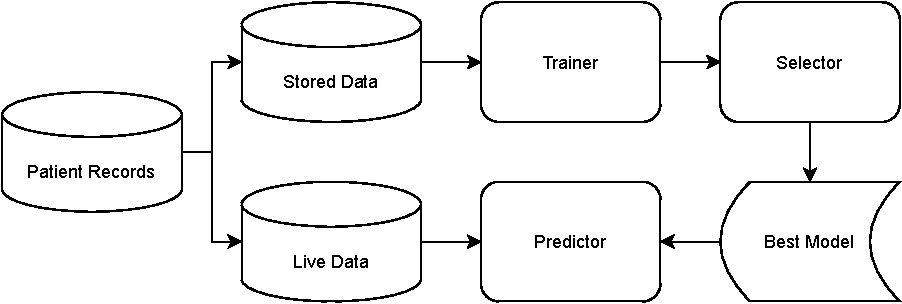
\includegraphics[width=0.7\columnwidth]{media/architecture/System Architecture.pdf}
    \caption{System architecture}
    \label{fig:system_architecture}
\end{figure}

\section{Data Flow in system}

The data used in this process goes through this sequential process shown in figure
\ref{fig:data_flow_in_system}

\begin{figure}[H]
    \centering
    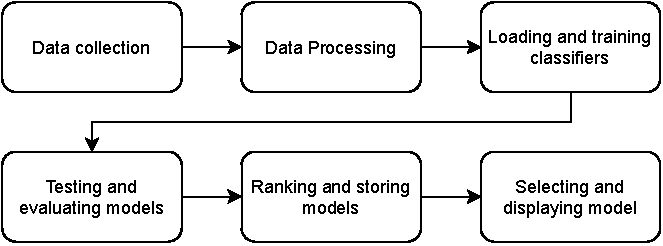
\includegraphics[width=0.7\columnwidth]{media/website/architecture/Data_Flow_System.pdf}
    \caption{Training and Selection Process}
    \label{fig:data_flow_in_system}
\end{figure}

\textbf{Data collection:} Collection of data is the first step in this process. The data is
collected from the user. The data is stored in a local directory for further processing. The
data is then divided into training and testing sets.

\vspace{-0.5em}
\textbf{Data processing:} In this step data labels are converted to 1 or 0, with respect to
previous values. In case of data with more than 2 labels, labels with min value are converted
to 0 and other values are converted into 1.

\vspace{-0.5em}
\textbf{Loading and training classifiers:} In this step model templates are used for generation
of models. These models are trained with the help of processed training data.

\vspace{-0.5em}
\textbf{Testing and evaluating models:} The trained models are evaluated with help of processed
testing datasets. The performance metrics are stored for ranking models.

\vspace{-0.5em}
\textbf{Ranking and storing models:} Performance metrics obtained in previous steps are used to
rank the models, the models are stored in a local directory.

\vspace{-0.5em}
\textbf{Selecting and displaying model:} In this step rank of models are used for selection of
best model, this model is stored into best models directory for future predictions. The name of
this selected model is displayed to the user.

\section{Training and selection process} \label{sec:data_flow}

As shown in figure \ref{fig:training_and_selection_process}, the system is provided with a
dataset, in this case records of ECG reports of patients. This data is already provided with
labels. These labels can be boolean values i.e., 1 for True, and 0 for False, or they can have
a series of values starting from 0. This data is further divided into training dataset and
testing dataset. These datasets are forwarded to the extraction process. In the extraction
process, datasets labels are converted into 0 and 1, this will eliminate extra classes present
in labels by changing their value to 1. The processed training dataset is sent for the model
training. As soon as this process takes place, the training module accesses premade models
templates, and generates the model for training purposes. These models are trained with
processed training data and stored in a directory for evaluation purposes.

\begin{figure}[H]
    \centering
    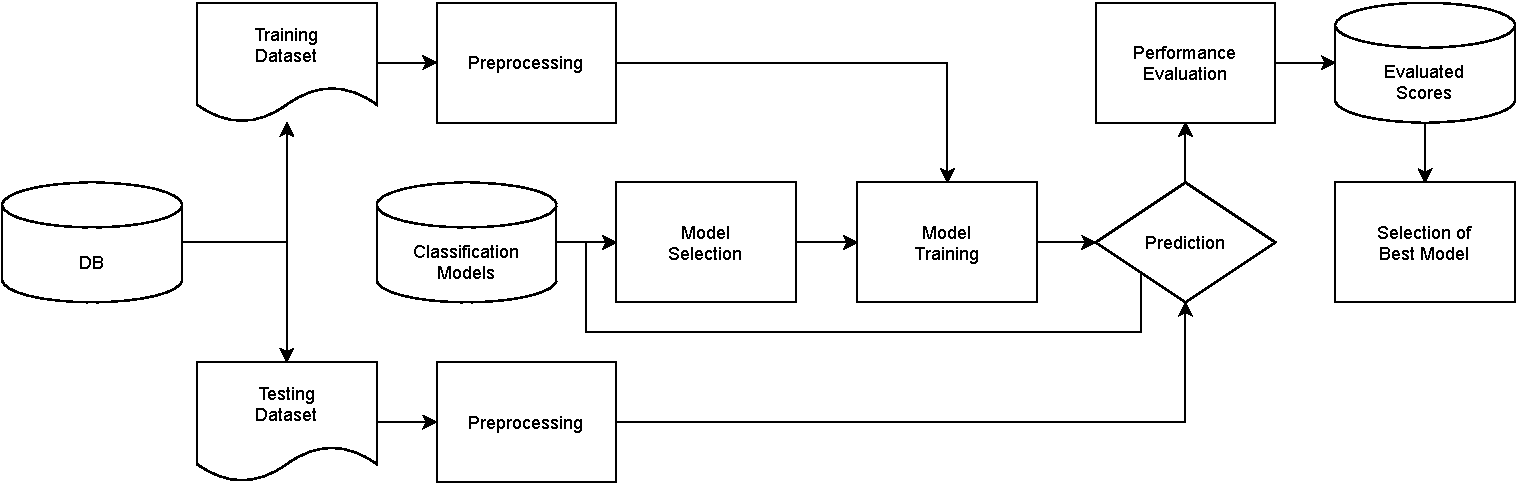
\includegraphics[width=0.9\columnwidth]{media/architecture/Process.pdf}
    \caption{Training and Selection Process}
    \label{fig:training_and_selection_process}
\end{figure}

Selector module accesses the stored models and processed testing dataset to evaluate the
performance of models. The performance metrics used for evaluation are accuracy score, f1
score, precision score, recall score, roc score and prediction time of model. These parameters
are multiplied with default or user provided weightage provided to generate scores of the
models. These scores are stored and used to select the best suited model.

\section{Machine Learning Terminology} \label{sec:machine_learning_terminology}


\section{Classifiers Used} \label{sec:supervised_learning}

The classifiers are algorithms that classify data into two or more classes based on rules set
out by users. The models trained with these classifiers are used for classification purposes.
In this project we are using classifiers to train models, these models will output data into
two classes.

By default this system uses five different classifiers, they are K-Nearest Neighbors, Decision
Tree, Random Forest, Multilayer Perceptron and Support vector machines. These classifiers are
categorized as supervised learning algorithms or classifiers. These classifiers will predict
the classes of data provided by the user.

\subsection{K-Nearest Neighbors} \label{subsec:K_nearest_neighbors}

K-nearest neighbor (KNN) algorithm is a supervised machine learning algorithm. Classification
and regression problems such as multiclass problems are solved using this algorithm. KNN is
lazy learning and non-parametric algorithm, which can be advantages or disadvantages depending
on the user's requirements. These properties make this algorithm very effective and
uncomplicated in general tasks. The drawback of the simplicity is the slow prediction time.

\subsubsection{Algorithm for K-Nearest Neighbors:}
\begin{steps}
    \vspace{-0.5em}
    \setlength{\itemsep}{-0.2em}
    \item Determine the number of K neighbors.
    \item Determine the Euclidean distance between the K neighbors.
    \item Using the estimated Euclidean distance, find the K nearest neighbors.
    \item Count the number of data points in each category among these K neighbors.
    \item Assign new data points to the category with the greatest number of neighbors.
    \item The model is now complete.
    \vspace{-1em}
\end{steps}

\subsection{Decision Tree} \label{subsec:decision_tree}
Decision trees are the most popular and effective tool for classification and prediction. The
decision tree is a flow chart-like tree structure, where each internal node specifies a test
for the attribute, each branch represents the result of the test, and each leaf node contains
a class label. Decision trees are the most popular high-performance tool for classification and
prediction.

\subsubsection{Construction of Decision Trees:}
\vspace{-0.5em}
The trees are trained by subdividing the features into subsets based on the attribute values.
This process is run recursively on derived subsets. The recursion completes when all subsets of
nodes have the same value for the target variable or if the split doesn't add any additional
value to the prediction. Building a decision tree classifier is suitable for exploratory
knowledge discovery as it does not require domain knowledge or parameter adjustment. Decision
trees can handle high-dimensional data. In general, decision tree classifiers are more
accurate. Decision tree induction is a typical inductive approach to learning classification
knowledge.

\subsubsection{Alogrithm for Decision Trees:}
\begin{steps}
    \vspace{-0.5em}
    \setlength{\itemsep}{-0.2em}
    \item Start the tree on the root node that contains the complete dataset.
    \item Use the Attribute Selection Scale (ASM) to find the best attribute in the dataset.
    \item Divide S into a subset containing the possible values of the best attributes.
    \item Create a decision tree node with the best attributes.
    \item Recursively build a new decision tree using the subset of the dataset created in step
    3. Continue this process until you reach a stage where you can no longer classify the node,
    and you can call the last node a leaf node.
    \vspace{-1em}
\end{steps}

\subsection{Random Forest} \label{subsec:random_forest}
Random forest is a supervised learning algorithm based on a decision tree algorithm. This
algorithm generates multiple decision trees from the provided sample. These decision trees are
combined, and a majority vote is taken to solve the classification and regression problem. The
Random Forest classifier offers more accurate and stable predictions at a slightly slower
prediction time when compared with a decision tree.

\subsubsection{Bagging}
\vspace{-0.5em}
The random forest classifier is a type of ensemble classifier which uses the bagging technique.
Random samples from data sets are collected. These samples generate independent models. Random
forest uses decision tree classifiers for model generation. The final output is generated based
on majority voting after combining the results of all models. This process of combination and
majority voting is known as the aggregation process.

\subsubsection{Classification algorithm for Random Forest:}
\begin{steps}
    \vspace{-0.5em}
    \setlength{\itemsep}{-0.2em}
    \item N number of random records are taken from the dataset with k number of reports.
    \item Each sample generates a separate decision tree.
    \item Each decision tree will generate an output/prediction unrelated to other trees.
    \item The final output is determined based on majority voting in classification problems.
    \vspace{-1em}
\end{steps}

\subsection{Multi-layer Perceptron} \label{subsec:multi_layer_perceptron}
The multilayer perceptron is a neural network-based supervised learning algorithm. In this
network, input and output are not linearly mapped. It is a feedforward algorithm hence more
suitable for classification and regression problems. MLP uses a backpropagating algorithm for
training, making it faster and usable for general predictions.

\subsubsection{Construction of MLP}
\vspace{-0.5em}
The neural network is made up of three primary components, neuron, activation function, and
layers.

\vspace{-1em}
\textbf{Neuron:}
A neuron is the smallest unit of a neural network. It is based on neurons in the brain, which
take one or more inputs to produce an output. The inputs are weighted, and each neuron has
biases which are also weighted similar to inputs.

\vspace{-1em}
\textbf{Activation functions:}
The weighted sum of inputs and bias is passed through activation functions. This function
serves as a mapping between two layers. These functions are usually non-linear. Activation
functions control the firing of a neuron. We are using the sigmoid as an activation function.
The sigmoid function returns either a zero or postitive value.

\vspace{-1em}
\textbf{Layers:}
Layers are rows of neurons in the network. The input layer is the entry point for the neural
network. The output layer serves as the exit point for the neural network. A hidden layer or
series of hidden layers connects input and output layers. In MLP, input layers take multiple
features as data. The output layer returns either 1 or 0.

\subsubsection{Algorithm for Multilayer Perceptron:}
\begin{steps}
    \vspace{-0.5em}
    \setlength{\itemsep}{-0.2em}
    \item N number of epochs is calculated by dividing sample size S by batch size B.
    \item Input layers accept the data features.
    \item Input layer forward data to hidden layers, which forward data to the output layer.
    \item Errors are calculated by comparing expected output and network output.
    \item The error propagated backward to adjust the weights of the network.
    \item All weights in the network are adjusted.
    \item Process in steps 3-6 is known as an epoch. The process is run for N number of epochs.
    \vspace{-1em}
\end{steps}

\vspace{-2em}
\subsection{Support Vector Machine} \label{subsec:support_vector_machine}
Support Vector Machines or SVM is one of the most commonly used supervised learning algorithms
for data classification and regression. This algorithm is primarily used to solve
classification problems in machine learning. The SVM algorithm created decision boundaries to
divide n-dimensional spaces into classes. The new data points are categorized using these
classes. The best boundary line which compartmentalizes most data accurately is called a
hyperplane. The SVM algorithm uses vectors to create the hyperplane. Support vectors handle
extreme cases giving the algorithm its name Support Vector Machine.

\vspace{-1em}
\textbf{Hyperplane:} A decision boundary separates new data points into different classes. The
decision boundary that produces the most accurate categorization is called the hyperplane. The
hyperplane adjusts with new data points by repositioning or introducing new dimensions.
Hyperplanes can be linear or non-linear, depending on user requirements.
 
\vspace{-1em}
\textbf{Support Vectors:} These are extreme data points present in data sets. Support vectors
have very close proximity to the hyperplane. Support vectors can directly affect the position
and dimensions of the hyperplane.

\subsubsection{Tuning parameters of SVM}
\vspace{-0.5em}
Tuning parameters used in this projects are:

\vspace{-1em}
\textbf{Kernal:} SVM uses the kernel function to solve problems. These functions allow smoother
operations on high dimensions. With kernels, SVM hyperplanes can theoretically reach infinite
dimensions. Kernels also reduce complexity at higher dimensions. The primary purpose of the
kernel is to provide a hyperplane way to accommodate non-linear datasets. In this project, we
are providing an RBF kernel. This kernel is suitable for both small and large quantities of
data.

\vspace{-1em}
\textbf{C parameter:} This is also known as the regularization parameter. C parameter suggests
SVM optimization amount of margin used by a hyperplane. A higher value of the C parameter 
produces accurate results. Conversely, a lower value results in fast but less accurate
predictions.

\vspace{-1em}
\textbf{Gamma:} The Gamma parameter defines the amount of influence of a model over the
dataset. Gamma is inversely proportional to the curve of influence of the model. Lower gamma
results in higher accuracy, but it is prone to overfitting. Higher gamma is constraining but
can't handle complexity.

% \begin{figure}[H]
%     \centering
%     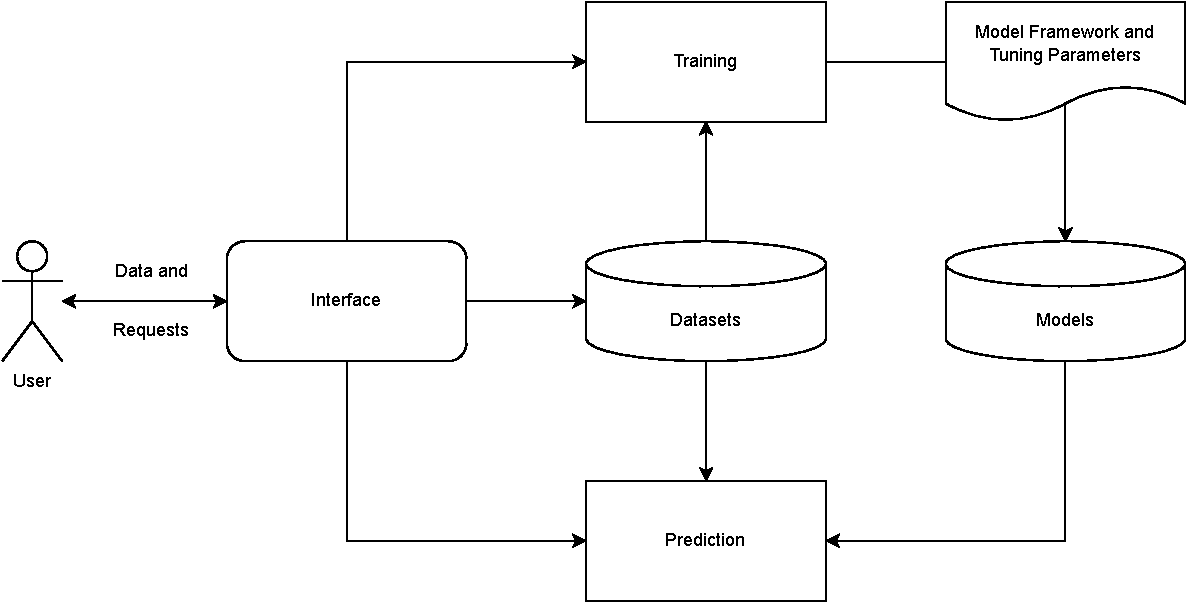
\includegraphics[width=0.9\columnwidth]{media/architecture/web_system_arch.pdf}
%     \caption{Web system architecture}
%     \label{fig:web_system_architecture}
% \end{figure}

\thispagestyle{fancy}
\chapter{System Interface} \label{ch:system_interface}
\section*{\centering Chapter \thechapter}
\section*{\centering System Interface}

The system takes data in CSV format. A web-based GUI will be offered to users. We are using a
flask-based web app for easier integration of the main system. We have implemented separate
pages for users depending on tasks. These pages are the selection page, prediction page,
performance page, and cross-performance page. We will see a detailed explanation of the pages
and the process carried out in the background.

\section{System Design} \label{sec:system_design}

The server is accessed with the help of a port number. The site is accessed by URL in the form
of \url{http://ip_address:port_number} URL syntax. In this development server we are using
\url{http} protocol and \url{127.0.0.1} or \url{localhost} as \url{ip_address}. The
\url{port_number} \url{5000} is used as per flask recommendation. Hence, the URL used by the
application to access the website is \url{http://localhost:5000}. In the next subsections, we
will go through each page available to the user.

\subsection{Login Page} \label{subsec:login_page}
This page is the first page encountered by a user when logging on to the website. This page
will take a valid username and password from the user and start the session for that username.
After starting the session, the user will be redirected to the Home page. Figure
\ref{fig:web_login_page} displays the login page.

\begin{figure}[H]
    \centering
    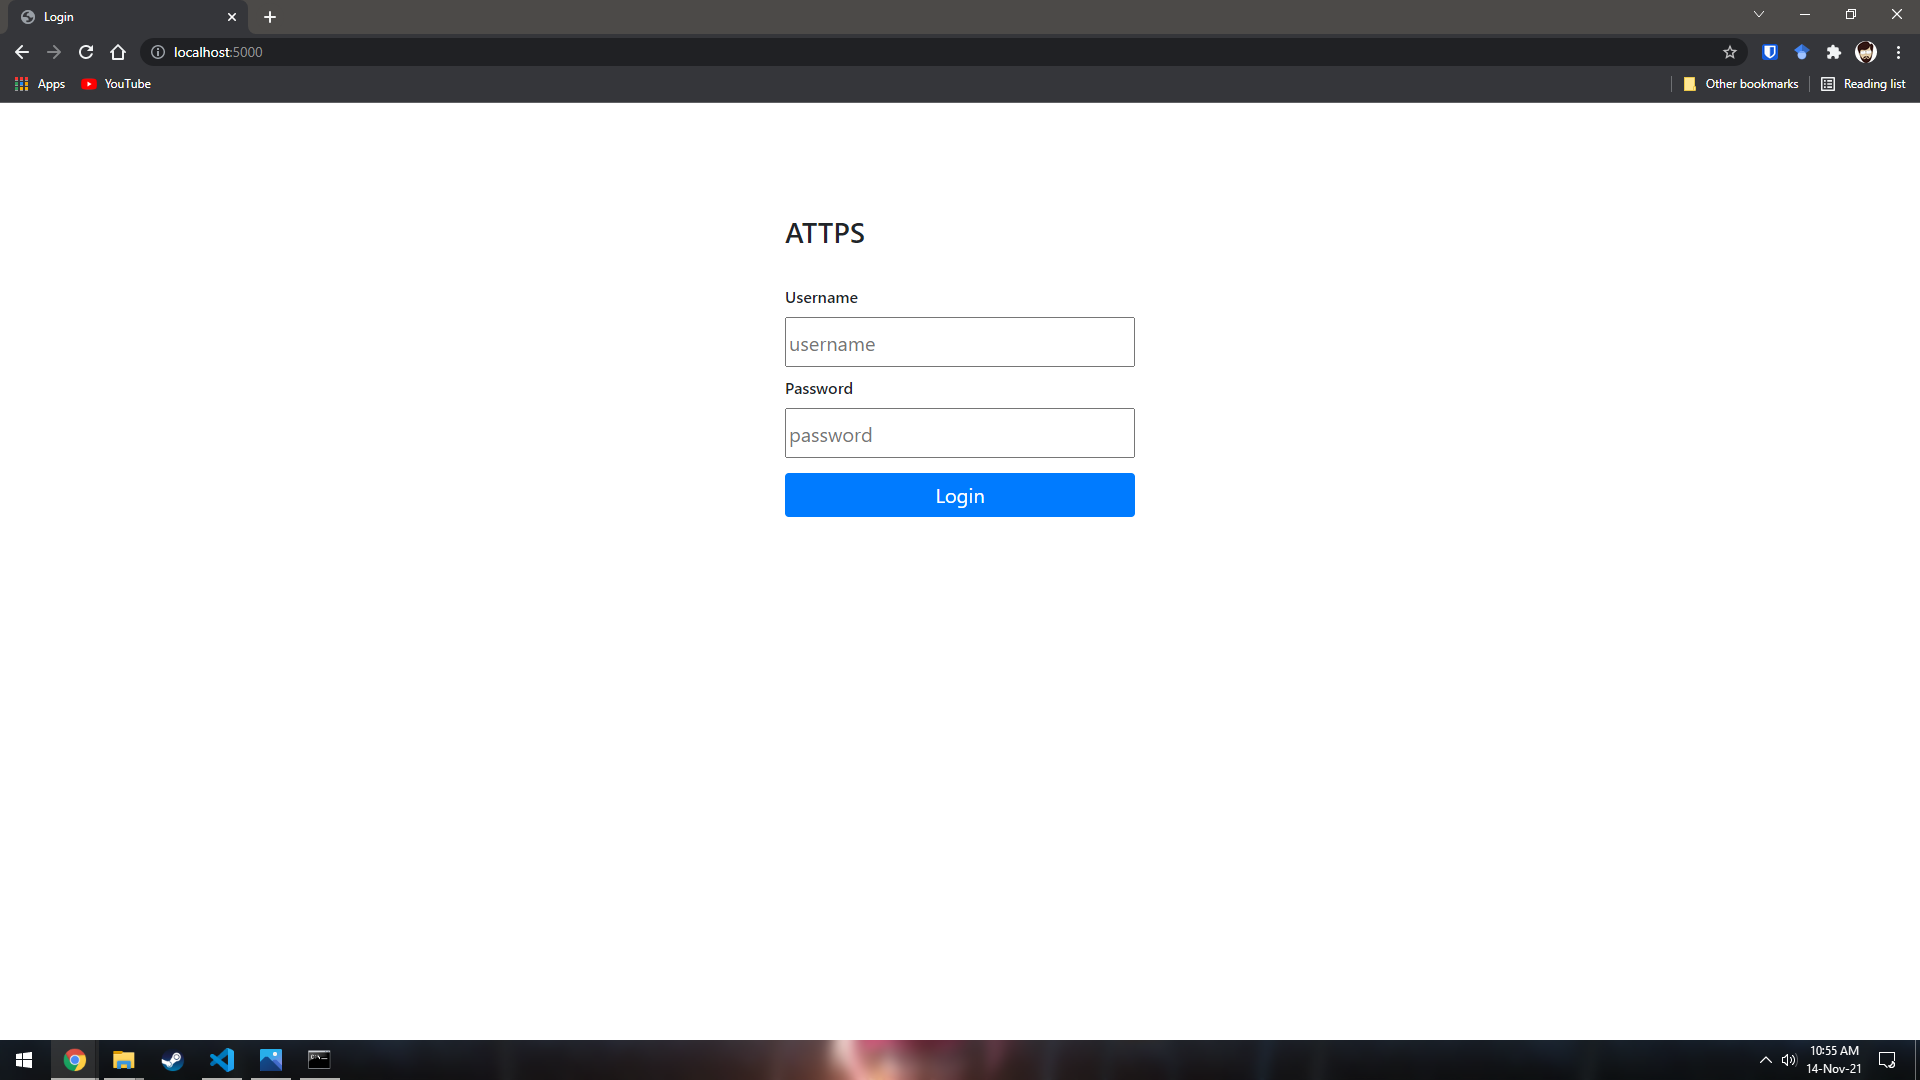
\includegraphics[width=0.7\columnwidth]{media/website/pages/00_login.png}
    \caption{Login Page}
    \label{fig:web_login_page}
\end{figure}

\subsection{Home Page} \label{subsec:home_page}
The home page is the landing page for the users after the session is started. It provides
information about the website. The side navigation is provided for users for easier access to
the rest of the website. This side navigation is present on all the pages except the login
page.

\subsection{Selector Page} \label{subsec:selector_page}
This page takes file input from the user. Currently, only CSV file format is supported. The
files are copied into the directory of the application. The training and selection module will
process the copied file. These modules will execute model training, performance evaluation, and
selection process. After process completion, the user will receive confirmation. Figure
\ref{fig:web_selector_page} displays the selector page.

\begin{figure}[H]
    \centering
    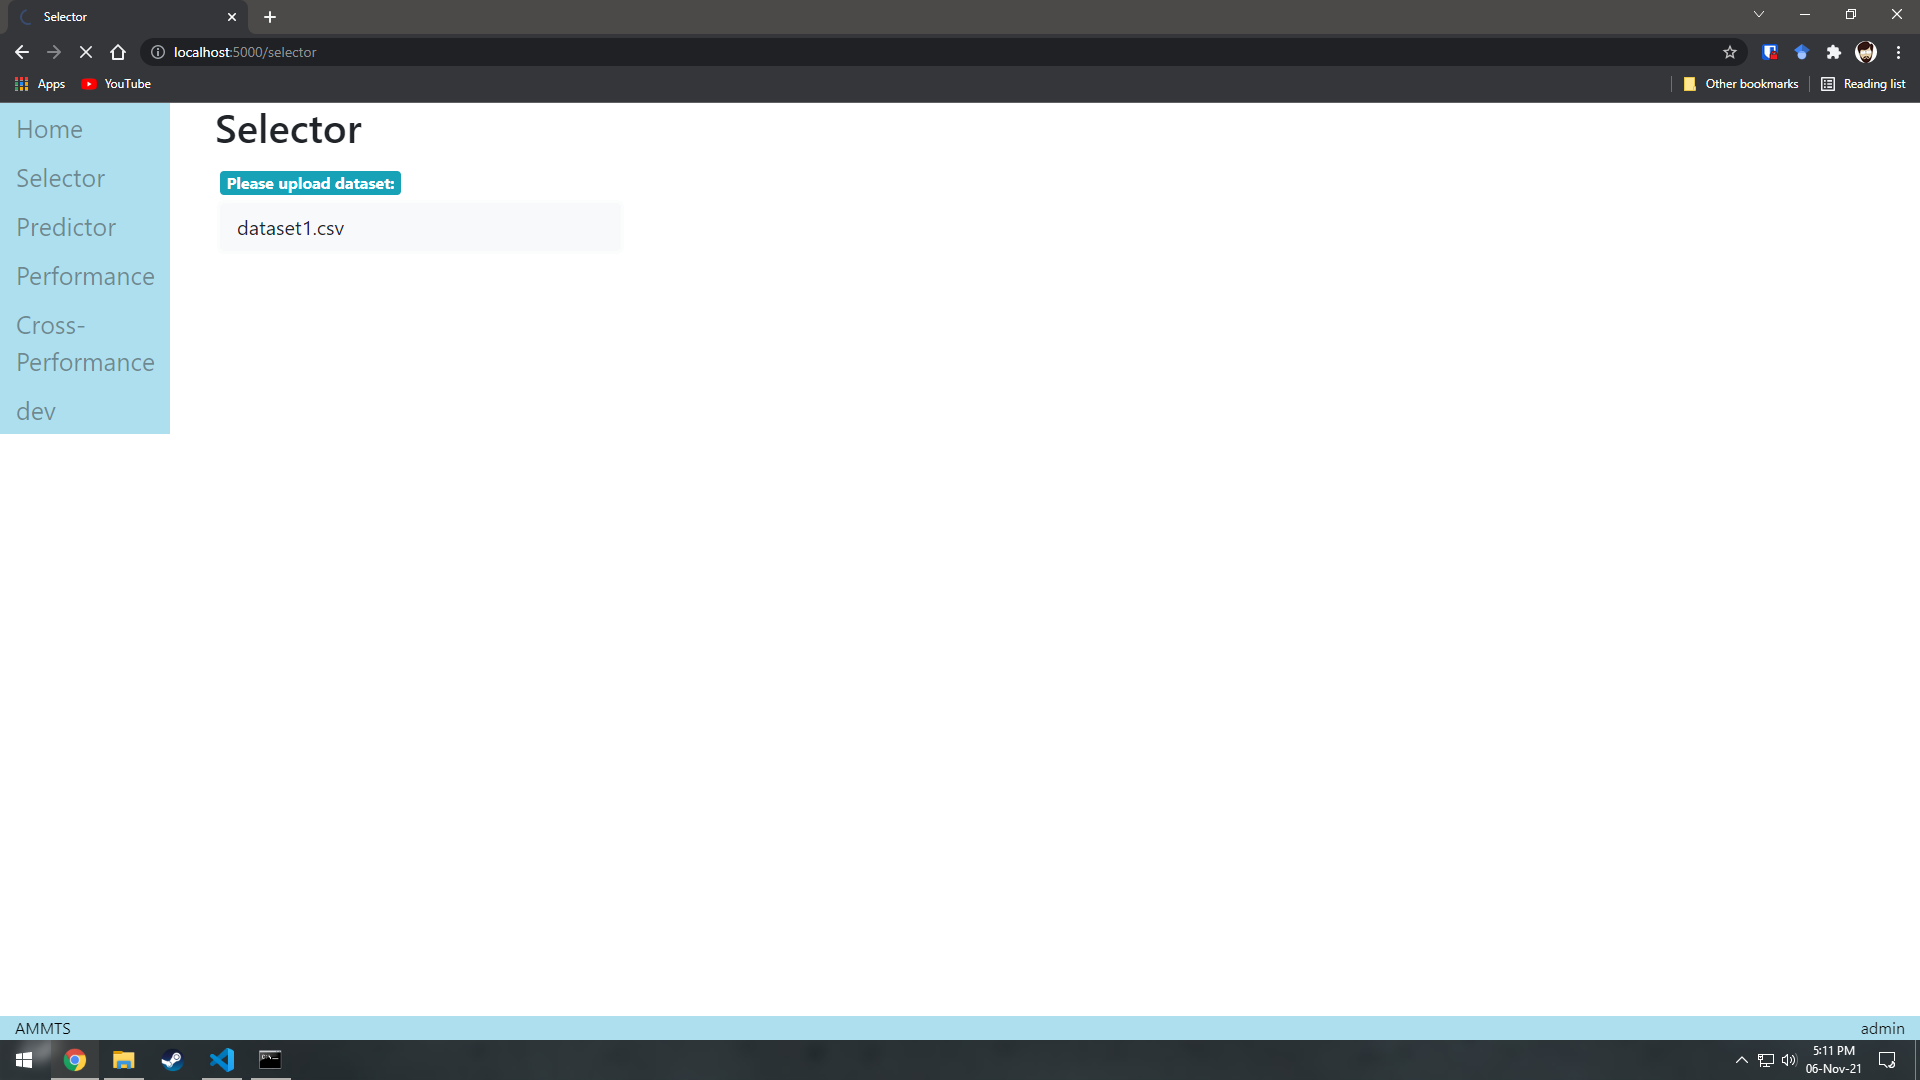
\includegraphics[width=0.7\columnwidth]{media/website/pages/02_selector.png}
    \caption{Selector Page}
    \label{fig:web_selector_page}
\end{figure}

\subsection{Selector-Upload Page} \label{subsec:selector_upload_page}
This page is a subpage to the selector page. This page is used to display the name of the
selected classifier to the user. This page has a similar layout to the selector page with a
small difference, and it acts similarly to the selector page. Figure
\ref{fig:web_selector_upload_page} displays the selector-upload subpage.

\begin{figure}[H]
    \centering
    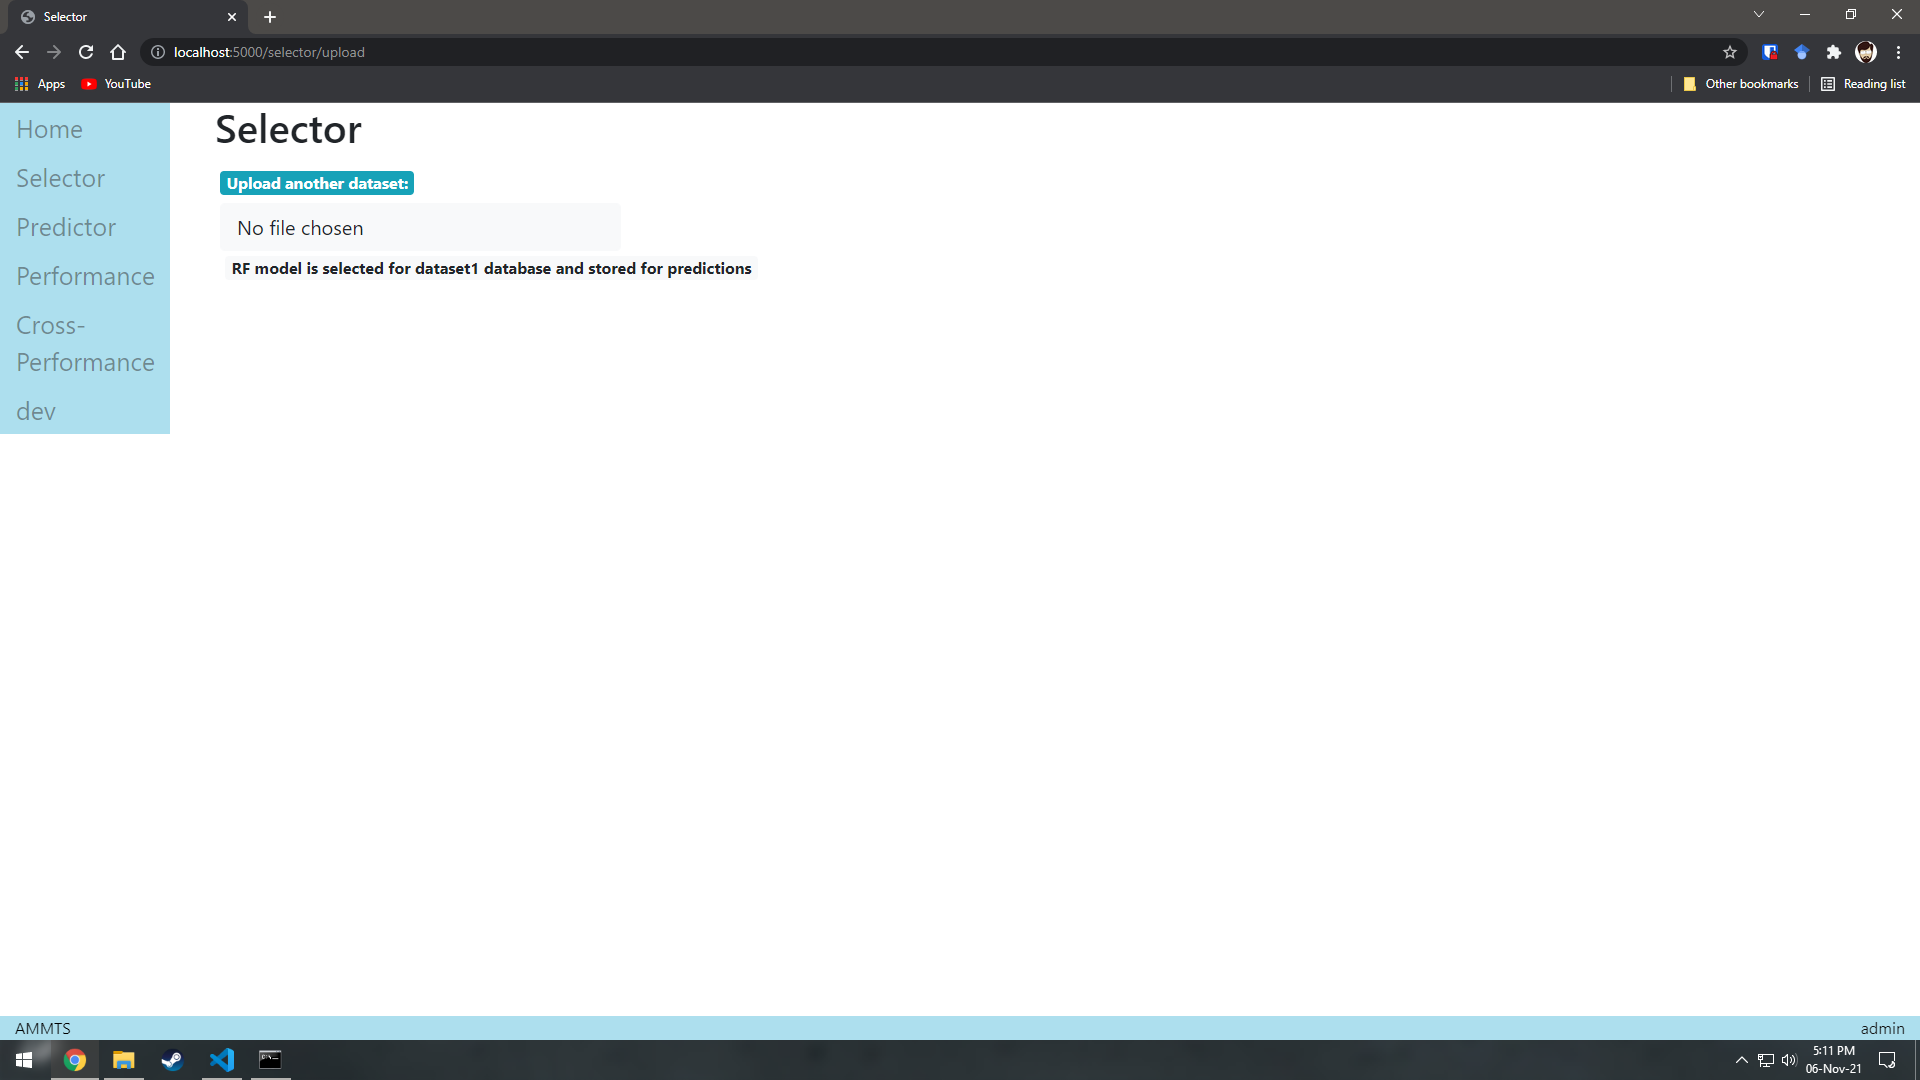
\includegraphics[width=0.7\columnwidth]{media/website/pages/02_selector_upload.png}
    \caption{Selector-Upload Page}
    \label{fig:web_selector_upload_page}
\end{figure}

\subsection{Predictor Page} \label{subsec:predictor_page}
This page is used to make predictions based on the dataset provided by the user. This page
generates a list of the best models for users to select models for predictions. The page also
generated a list of datasets provided by the user for predictions. If the dataset is not
available, the user is allowed to upload the dataset from the page. After submitting the
selected model and dataset page will run the prediction process on the datasets. After
completion of this process, the user is forwarded to the subpage. Figure
\ref{fig:web_predictor_page} displays the predictor page.

\begin{figure}[H]
    \centering
    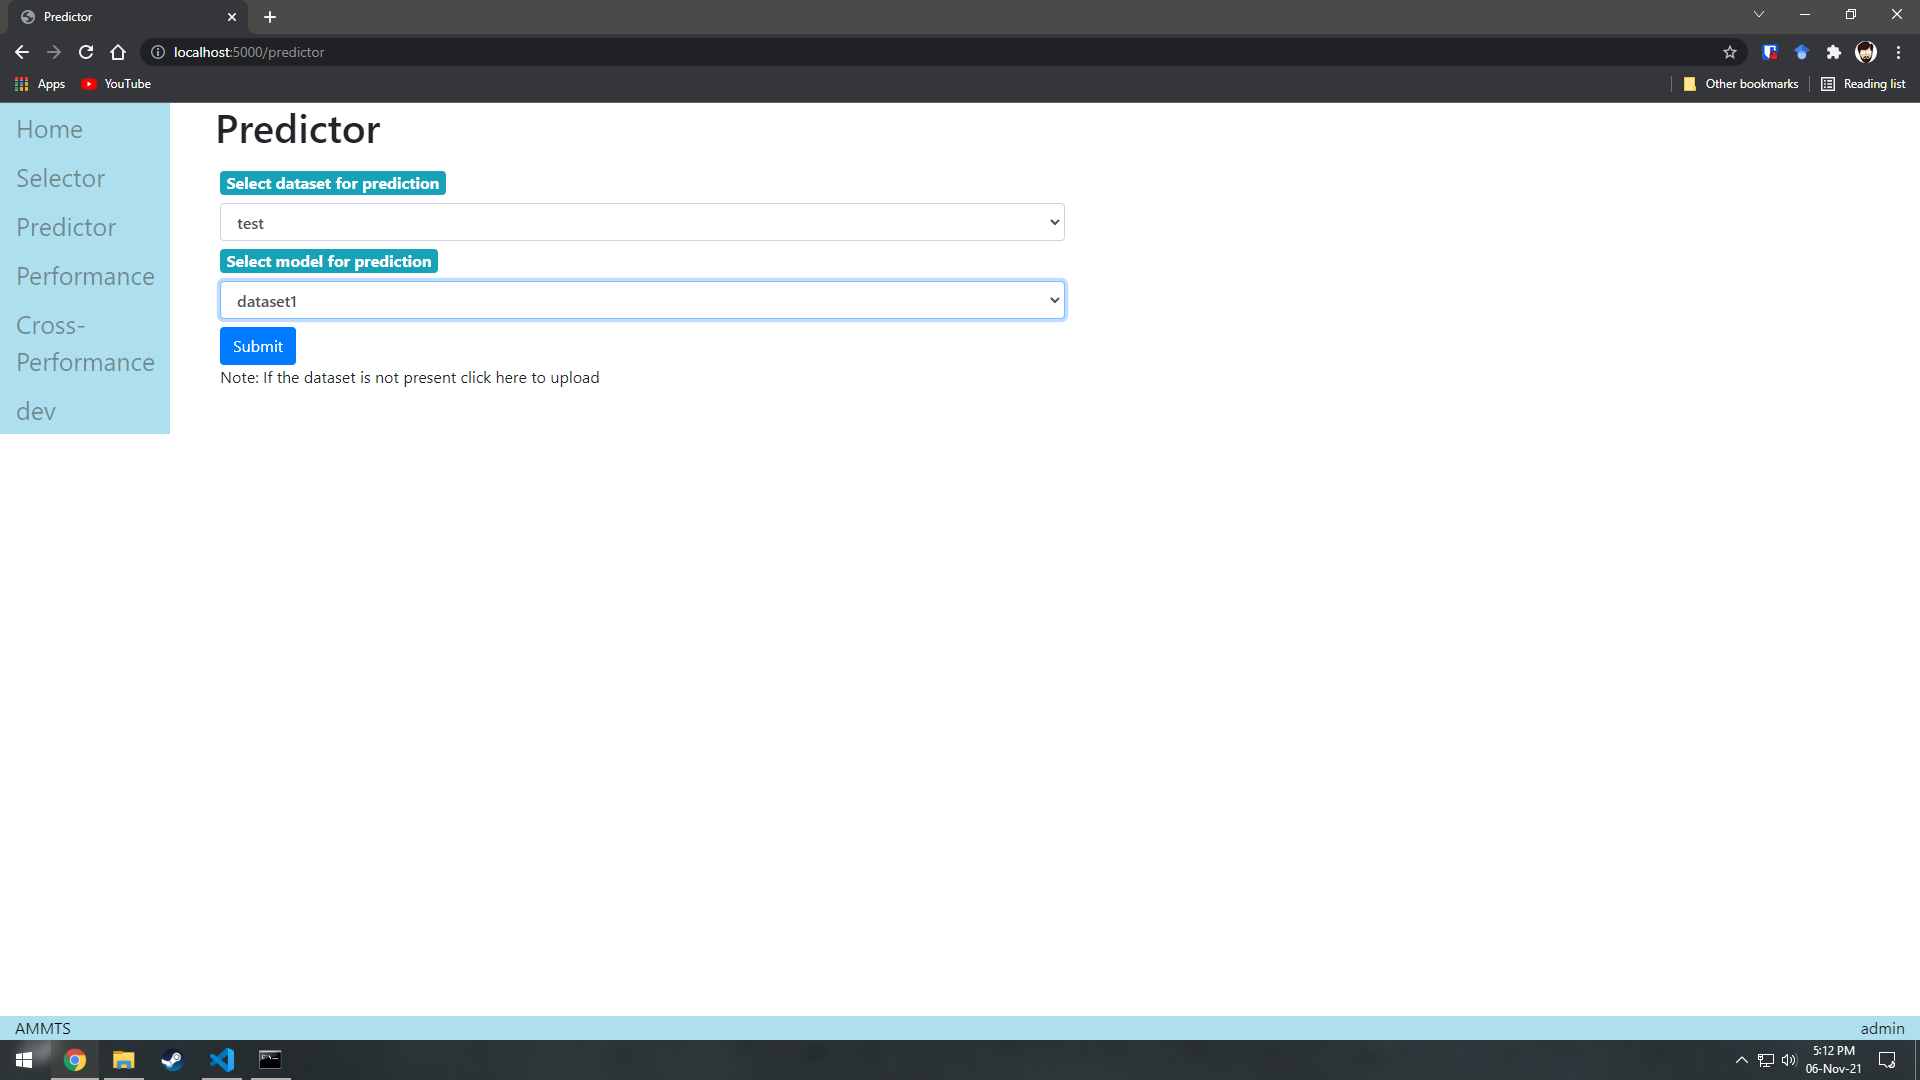
\includegraphics[width=0.7\columnwidth]{media/website/pages/03_predictor.png}
    \caption{Predictor Page}
    \label{fig:web_predictor_page}
\end{figure}

\subsection{Predictor-Results Page} \label{subsec:predictor_result_page}
This page will display the results of predictions obtained from the model and dataset submitted
by the user with the predictor page. The result is displayed in tabular format with ID and
prediction results as columns. Figure \ref{fig:web_predictor_results_page} displays the
predictor-results subpage.

\begin{figure}[H]
    \centering
    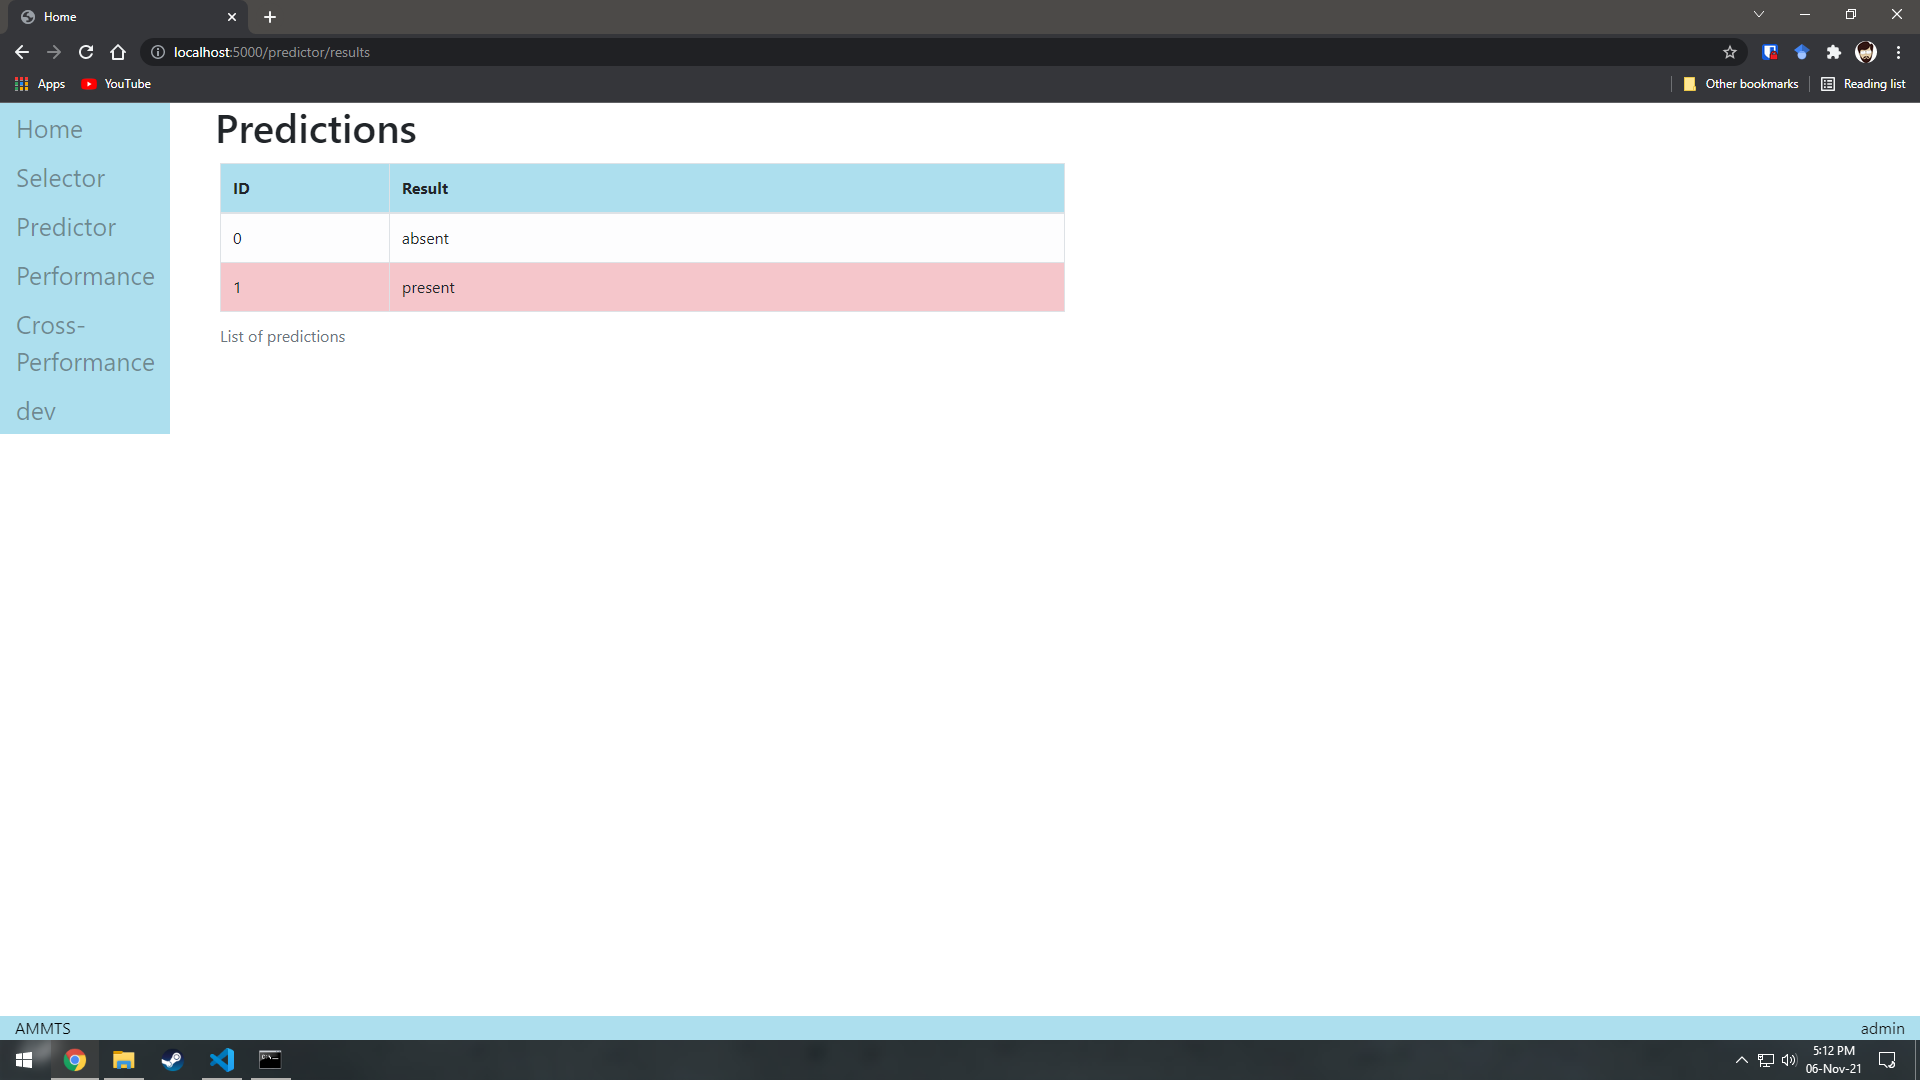
\includegraphics[width=0.7\columnwidth]{media/website/pages/03_predictor_results.png}
    \caption{Predictor-Results Page}
    \label{fig:web_predictor_results_page}
\end{figure}

\subsection{Performance Page} \label{subsec:performance_page}
This page allows users to select models from a list of models created from previous datasets.
After selecting the model, the page will get performance data stored in the local directory and
redirect the user to the subpage. Figure \ref{fig:web_performance_page} displays the
performance page.

\begin{figure}[H]
    \centering
    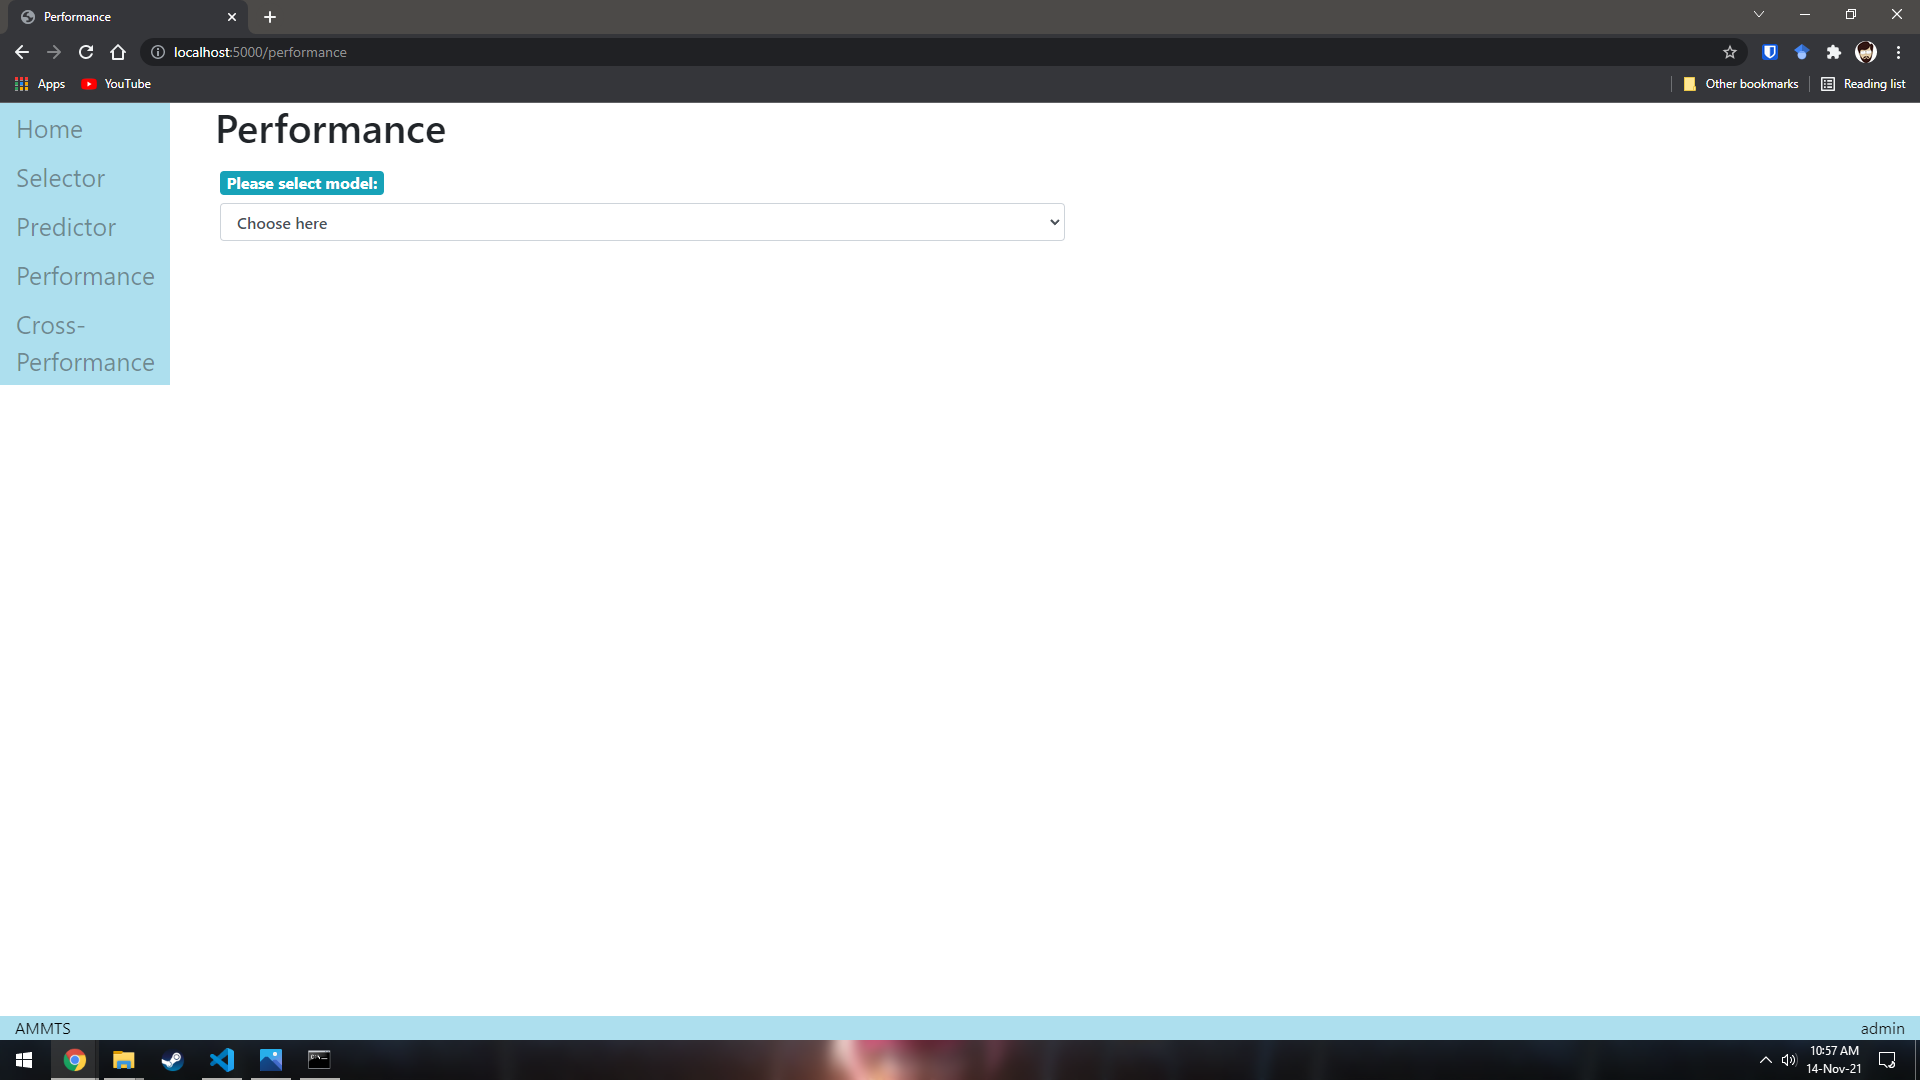
\includegraphics[width=0.7\columnwidth]{media/website/pages/04_Performance.png}
    \caption{Performance Page}
    \label{fig:web_performance_page}
\end{figure}

\subsection{Performance-Display Page} \label{subsec:performance_display_page}
This page will display the performance obtained from the performance page. This page has a
similar base layout to the performance page and has an option to display the graph generated
from performance. This page also acts similar to the performance page. It allows the user to
select another model to display its performance. Figure \ref{subsec:performance_display_page}
displays the performance-display page.

\begin{figure}[H]
    \centering
    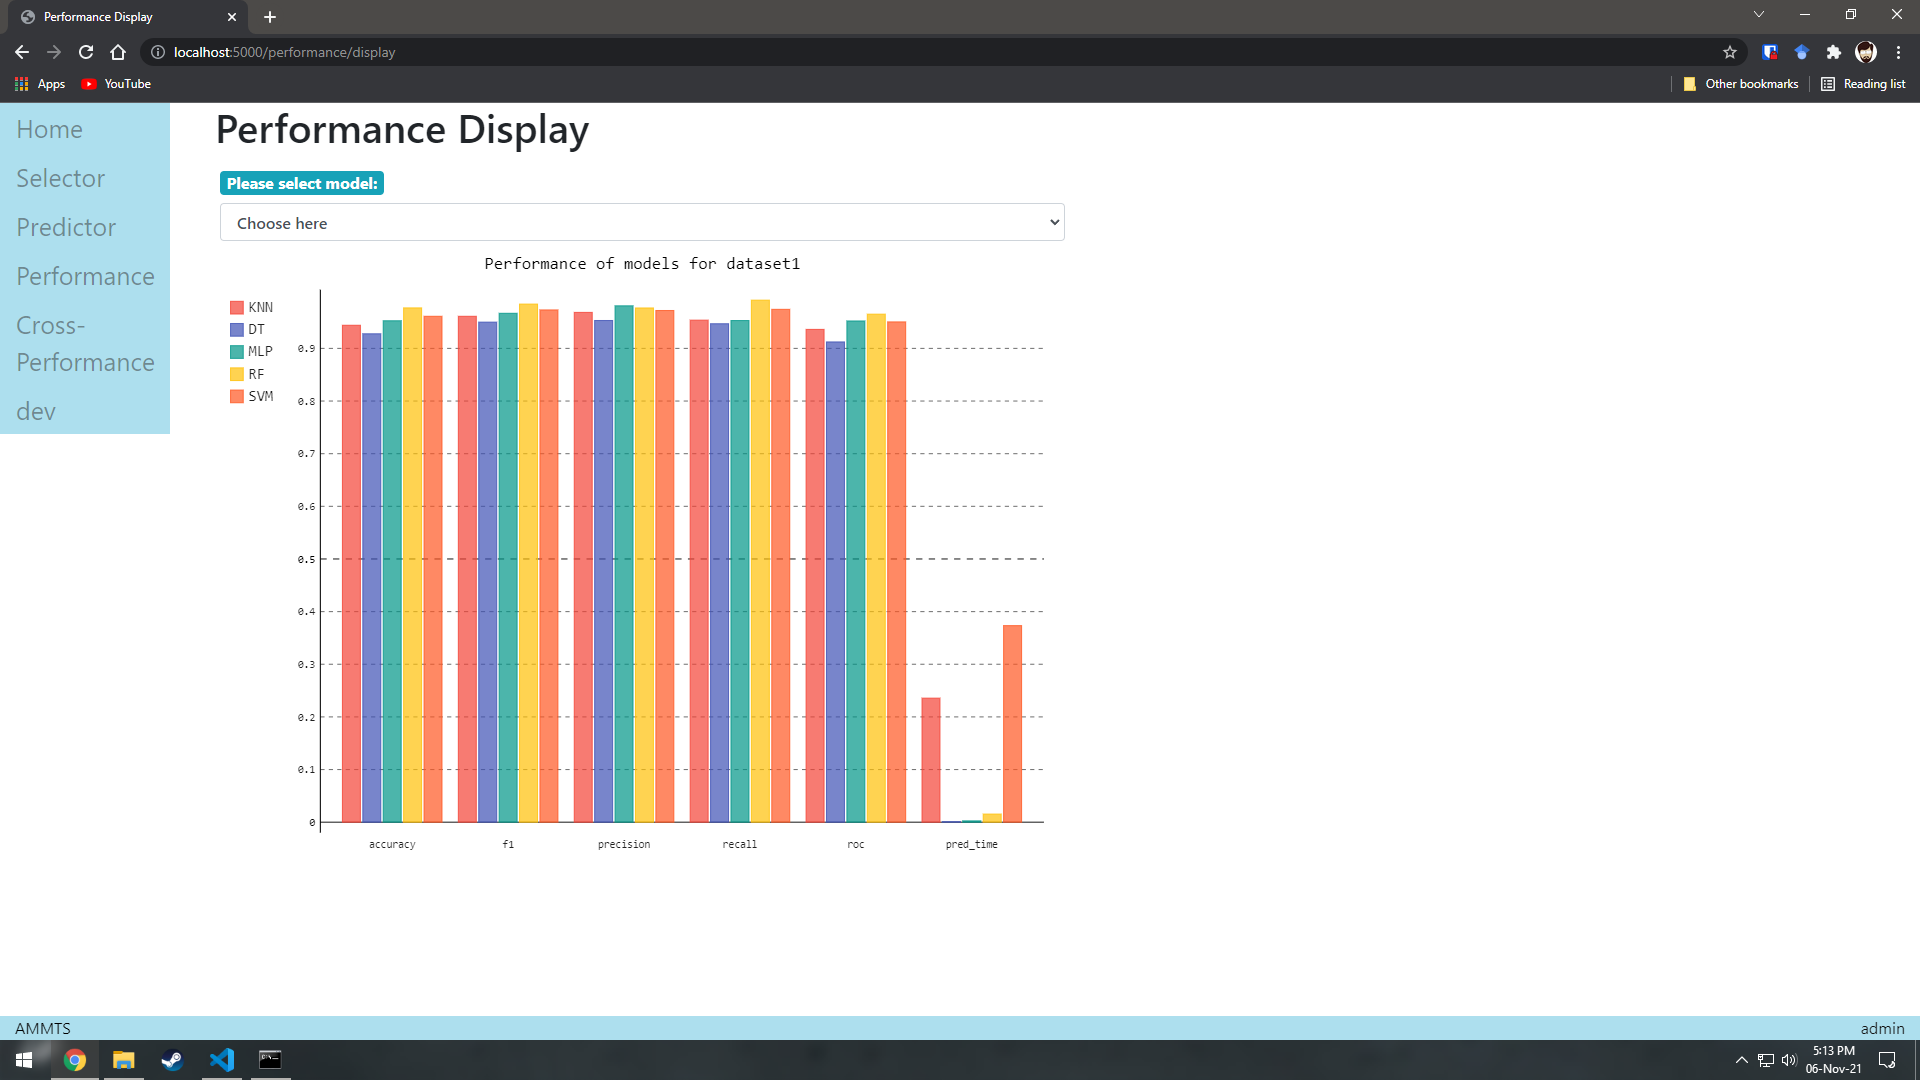
\includegraphics[width=0.7\columnwidth]{media/website/pages/04_performance_display.png}
    \caption{Performance-Display Page}
    \label{fig:web_performance_display_page}
\end{figure}

\subsection{Cross-Performance Page} \label{subsec:cross_performance_page}
This page allows users to select models from a list of models created from previous datasets.
The page also provides a list of datasets uploaded by the user for predictions. The user is
required to select a dataset from this list. The user-selected dataset and model will be sent
to the server for cross-performance analysis. After completion of the cross-performance
process, the user is redirected to the subpage. Figure \ref{fig:web_cross_performance_page}
displays cross-performance page.

\begin{figure}[H]
    \centering
    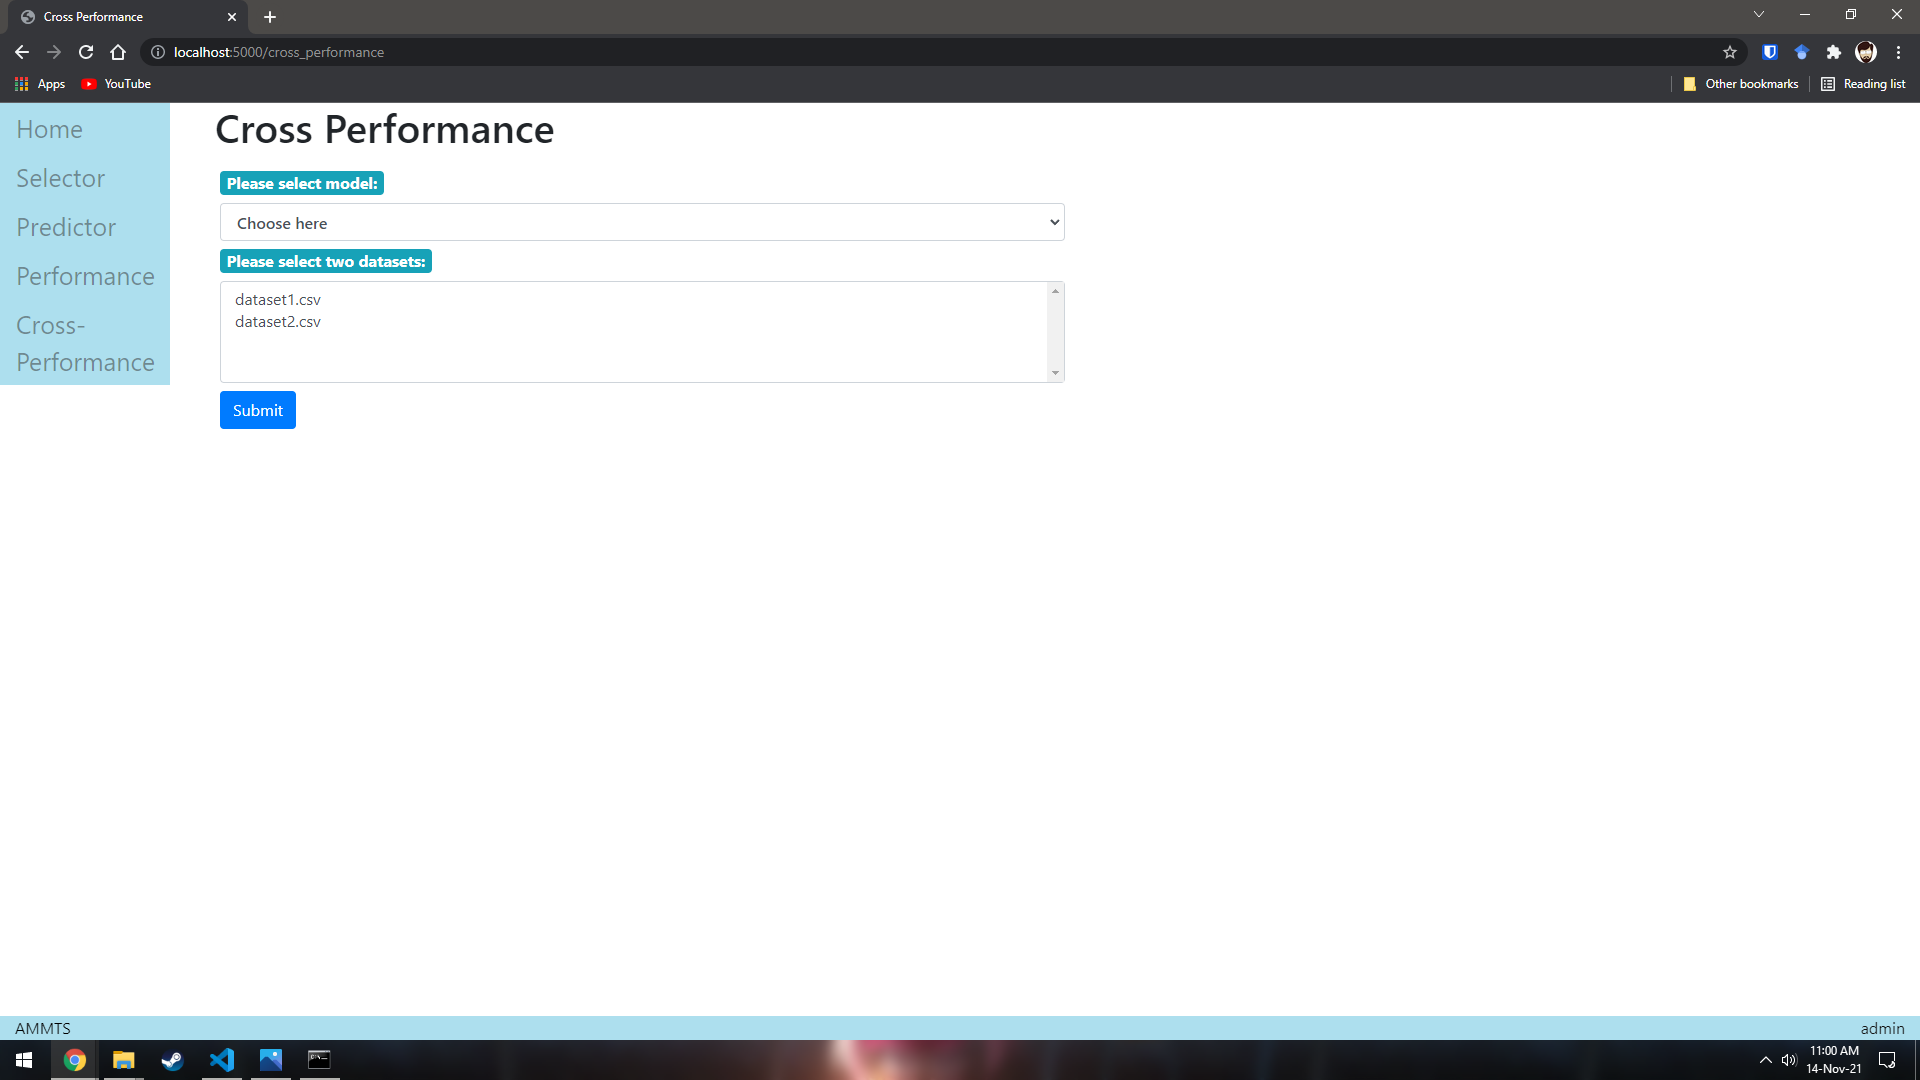
\includegraphics[width=0.7\columnwidth]{media/website/pages/05_cross_performance.png}
    \caption{Cross-Performance Page}
    \label{fig:web_cross_performance_page}
\end{figure}

\subsection{Cross-Performance-Display Page} \label{subsec:cross_performance_display Page}
This page will receive the data obtained from the cross-performance process and display the
data in chart format. This page has a similar layout and acts similar to a cross-performance
page, with a display place for charts. Figure \ref{fig:web_cross_performance_display_page}
displays the cross-performance-display page.

\begin{figure}[H]
    \centering
    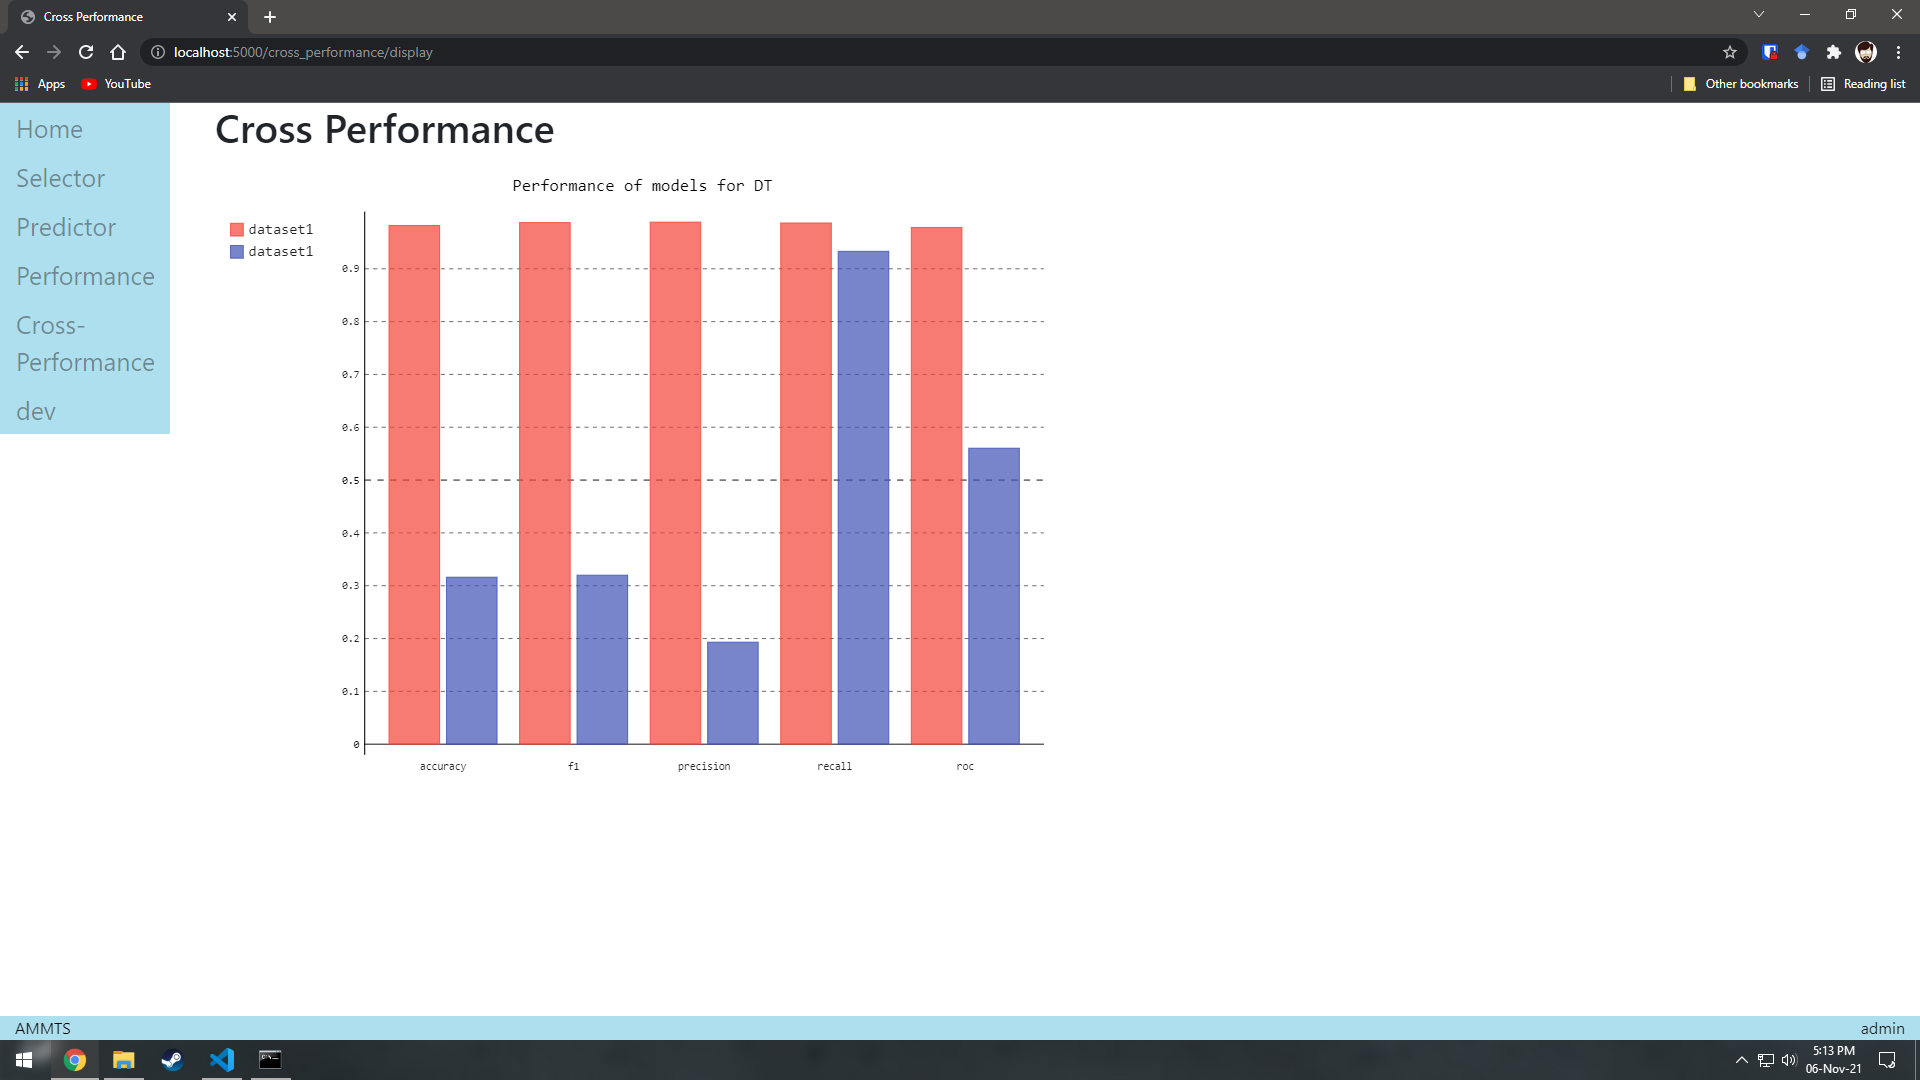
\includegraphics[width=0.7\columnwidth]{media/website/pages/05_cross_performance_display.png}
    \caption{Cross-Performance-Display Page}
    \label{fig:web_cross_performance_display_page}
\end{figure}

\subsection{Helper Pages} \label{subsec:helper_page}
These pages act as helper pages for users as well as handles errors. In the instance of
unauthorized access or invalid information, users are redirected to these pages.

\section{Hardware Details} \label{sec:hardware_details}
The hardware used for the program is given below. The system needs at least a moderate amount
of memory for operations. The amount of system memory used during development is 16 GB. The
system also needs a high-performance CPU for the model training. The number of cores available
for calculation is important too. The development system uses a 3.6 GHz processor with 6 Cores.
The data uploaded by users and system-generated data need storage space. The recommended size
of the storage is 250 GB.

Standard input and output devices are required to take data and commands from users and display
them.

\begin{table}[H]
    \centering
    \caption{Hardware Details} \label{tab:hardware_details}
    \begin{tabular}{|L{10em}|L{25em}|}
        \hline
        \textbf{Hardware} & \textbf{Details}
        \rule[-2ex]{0pt}{4ex}\\\hline
        Installed memory (RAM) & 16.00 GB
        \rule[-2ex]{0pt}{4ex}\\\hline
        Storage & 250 GB SSD
        \rule[-2ex]{0pt}{4ex}\\\hline
        Processor & AMD Ryzen 5 3500 6-Core Processor 3.6 GHz
        \rule[-2ex]{0pt}{4ex}\\\hline
        GPU & NVIDIA GeForce GTX 1650 Super
        \rule[-2ex]{0pt}{4ex}\\\hline
        Input device & Standard Keyboard and Mouse
        \rule[-2ex]{0pt}{4ex}\\\hline
    \end{tabular}
\end{table}

\section{Software Details} \label{sec:software_details}
The software requirements of the application are described below. The application is developed
on Windows 10 system, but it is OS independent application. The technologies used are python as
a base programming language, sklearn library to make model templates, and flask to develop the
web application. Pandas library is used for data handling. HTML, CSS, and JavaScript are used
for web pages.

\begin{table}[H]
    \centering
    \caption{Software Requirement} \label{tab:software_requirement}
        \begin{tabular}{|L{10em}|L{25em}|}
        \hline
        \textbf{Software} & \textbf{Details}
        \rule[-3ex]{0pt}{6ex}\\\hline
        Operating System & Windows 10
        \rule[-2ex]{0pt}{4ex}\\\hline
        Technology & Python, Scikit-learn, Pandas, Flask, HTML, JavaScript
        \rule[-2ex]{0pt}{4ex}\\\hline
    \end{tabular}
\end{table}
\thispagestyle{fancy}
\chapter{Result And Analysis} \label{ch:result_and_analysis}
\section*{\centering Chapter \thechapter}
\section*{\centering Result And Analysis}


\section{Performance Measures} \label{sec:performance_measures}
There are a lot of different types of parameters to evaluate the performance of machine learning models. In case of the classification models Accuracy score, F1 score, Recall score, Precision score and total area under ROC curve used for performance evaluation.

\subsection{Accuracy Score}\label{subsec:accuracy_score}
The accuracy score is a fraction of the correct prediction by model with respect to total predictions by model. It can be represented by following formula:

\begin{equation}\label{eq:accuracy_score}
  Accuracy = \frac{TP+TN}{TP+TN+FP+FN}
\end{equation}
\myequations{Accuracy Score}

\subsection{Precision score}\label{subsec:precision_score}
The precision score is a fraction of the correct positive predictions with respect to all positive predictions of the model. Higher precision scores result in fewer false positive predictions. It can be represented by following formula:

\begin{equation}\label{eq:precision_score}
  Precision = \frac{TP}{TP+FP}
\end{equation}
\myequations{Precision Score}

\subsection{Recall score}\label{subsec:recall_score}
The recall score is the fraction of correct positive predictions with respect to all predictions of the class. It can be represented by following formula:

\begin{equation}\label{eq:recall_score}
  Recall = \frac{TP}{TP+FN}
\end{equation}
\myequations{Recall Score}

\subsection{F1 score}\label{subsec:f1_score}
The F1 score is the weighted average of the recall score and precision score of the model. F1 scores are more reliable than accuracy scores in case of biased or uneven dataset. It can be represented by following formula:

\begin{equation}\label{eq:f1_score}
  F1 = 2 \cdot \frac{Recall \cdot Precision}{Recall + Precision}
\end{equation}
\myequations{F1 Score}

F1 score can also be represented as
$F1 = \frac{TP}{TP+\frac{1}{2}(FP+FN)}$

\subsection{AUC ROC score}\label{subsec:auc_roc_score}
The ROC is a classifier's predictive quality that compares and visualizes the trade-off between the model's sensitivity and specificity. In graphical format, the area under it gives a relationship between false positives and true positives. The higher these areas are, the better the predictive quality of the model.

\subsection{Prediction Time}\label{subsec:prediction_time}
Prediction times are nothing but the amount of time required by the classifier to make predictions for certain testing datasets. A model with a lower prediction time is desirable.

\subsection{Performance Evaluation Methodology} \label{subsec:performance_evaluation_methodology}
Performance scores are calculated with performance evaluation metrics and average prediction time. The models are ranked based on performance scores.

Weighted sums of the ranks are stored for the selection process. Weightage is predefined. It lies between 0 to 1, and it is directly proportional to the significance of the metric. For example, in situations where speed is more important than accuracy, prediction time is given higher weightage than accuracy metrics.

In the proposed system lowest scoring model is selected as the ideal model.

\section{Dataset Description} \label{sec:dataset_description}
The goal of the project is to detect the presence of arrhythmia from ECG signals accurately and faster than the traditional approach. For this task, a well-known open-access database MIT-BIH Arrhythmia Training and Testing Dataset are used. Both datasets are divided into four equal parts randomly and used for training and testing respectively. Each training set contains 21888 signals and the testing set contains 5473 signals.

\section{Performance Evaluation} \label{sec:performance_evaluation}
The datasets obtained from the MIT-BIH training dataset showed significant similarities in performance evaluation. All four datasets showed higher performance metrics for SVM classifiers. The prediction time required by SVM and KNN was significantly higher than other classifiers. The desired result can be tweaking ranking parameters. The performance of models is shown in \cref{fig:perfromance_results}.

\Cref{tab:performance_of_models_trained_on_dataset_1} shows the Random Forest model have highest Vscore for dataset 1, hence it is selected as the most-suited model for this dataset. While \cref{tab:performance_of_models_trained_on_dataset_2,tab:performance_of_models_trained_on_dataset_3,tab:performance_of_models_trained_on_dataset_4} shows the Support Vector Machine model scored higher Vscore for other three datasets, hence it has been chosen as most-suited model for those datasets. \Cref{tab:v_score_of_models} shows the V$_{score}$ of all models.

% ************** Performance of models trained on dataset 1, 2, 3, and 4 tabular **************
% ***************************************** Dataset 1 *****************************************
\begin{table}[H]
  \centering
  \caption{Performance of models trained on Dataset 1}\label{tab:performance_of_models_trained_on_dataset_1}
  \begin{tabular}{|p{5em}|C{3em}|C{3em}|C{3em}|C{3em}|C{3em}|}
    \hline
    \textbf{Metric}      & \textbf{KNN} & \textbf{DT} & \textbf{MLP} & \textbf{RF}    & \textbf{SVM} \\
    \hline
    \textbf{Accuracy}    & 96.72        & 94.46       & 96.89        & \textbf{97.33} & 97.40        \\
    \textbf{F1}          & 89.71        & 83.43       & 90.05        & \textbf{91.30} & 91.69        \\
    \textbf{Precision}   & 92.53        & 81.86       & 94.71        & \textbf{97.95} & 96.43        \\
    \textbf{Recall}      & 87.06        & 85.06       & 85.84        & \textbf{85.50} & 87.40        \\
    \textbf{ROC}         & 92.84        & 90.68       & 92.45        & \textbf{92.57} & 93.38        \\
    \textbf{Time(s)}     & 0.457        & 0.001       & 0.002        & \textbf{0.015} & 0.297        \\
    \textbf{V$_{score}$} & 2.747        & 2.643       & 2.782        & \textbf{2.807} & 2.482        \\
    \hline
  \end{tabular}
\end{table}

% ***************************************** Dataset 2 *****************************************
\begin{table}[H]
  \centering
  \caption{Performance of models trained on Dataset 2}\label{tab:performance_of_models_trained_on_dataset_2}
  \begin{tabular}{|p{5em}|C{3em}|C{3em}|C{3em}|C{3em}|C{3em}|}
    \hline
    \textbf{Metric}      & \textbf{KNN} & \textbf{DT} & \textbf{MLP} & \textbf{RF} & \textbf{SVM}   \\
    \hline
    \textbf{Accuracy}    & 96.83        & 95.04       & 96.69        & 97.09       & \textbf{97.46} \\
    \textbf{F1}          & 90.28        & 85.50       & 89.73        & 90.75       & \textbf{92.15} \\
    \textbf{Precision}   & 94.25        & 84.90       & 94.73        & 98.60       & \textbf{96.79} \\
    \textbf{Recall}      & 86.63        & 86.09       & 85.23        & 84.05       & \textbf{87.93} \\
    \textbf{ROC}         & 92.77        & 91.48       & 92.13        & 91.90       & \textbf{93.66} \\
    \textbf{Time(s)}     & 0.435        & 0.001       & 0.003        & 0.014       & \textbf{0.295} \\
    \textbf{V$_{score}$} & 2.758        & 2.684       & 2.772        & 2.795       & \textbf{2.808} \\
    \hline
  \end{tabular}
\end{table}

% ***************************************** Dataset 3 *****************************************
\begin{table}[H]
  \centering
  \caption{Performance of models trained on Dataset 3}\label{tab:performance_of_models_trained_on_dataset_3}
  \begin{tabular}{|p{5em}|C{3em}|C{3em}|C{3em}|C{3em}|C{3em}|}
    \hline
    \textbf{Metric}      & \textbf{KNN} & \textbf{DT} & \textbf{MLP} & \textbf{RF} & \textbf{SVM}   \\
    \hline
    \textbf{Accuracy}    & 97.07        & 94.64       & 96.41        & 97.22       & \textbf{97.44} \\
    \textbf{F1}          & 90.93        & 84.30       & 89.34        & 91.21       & \textbf{92.00} \\
    \textbf{Precision}   & 95.82        & 83.81       & 90.13        & 98.37       & \textbf{97.81} \\
    \textbf{Recall}      & 86.53        & 84.80       & 88.57        & 85.02       & \textbf{86.85} \\
    \textbf{ROC}         & 92.87        & 90.73       & 93.29        & 92.36       & \textbf{93.22} \\
    \textbf{Time(s)}     & 0.404        & 0.001       & 0.002        & 0.017       & \textbf{0.293} \\
    \textbf{V$_{score}$} & 2.774        & 2.658       & 2.766        & 2.803       & \textbf{2.803} \\
    \hline
  \end{tabular}
\end{table}

% ***************************************** Dataset 4 *****************************************
\begin{table}[H]
  \centering
  \caption{Performance of models trained on Dataset 4}\label{tab:performance_of_models_trained_on_dataset_4}
  \begin{tabular}{|p{5em}|C{3em}|C{3em}|C{3em}|C{3em}|C{3em}|}
    \hline
    \textbf{Metric}      & \textbf{KNN} & \textbf{DT} & \textbf{MLP} & \textbf{RF} & \textbf{SVM}   \\
    \hline
    \textbf{Accuracy}    & 96.84        & 94.99       & 95.34        & 96.88       & \textbf{97.15} \\
    \textbf{F1}          & 90.52        & 85.73       & 85.01        & 90.37       & \textbf{91.39} \\
    \textbf{Precision}   & 95.71        & 85.91       & 97.83        & 98.65       & \textbf{97.41} \\
    \textbf{Recall}      & 85.86        & 85.55       & 75.15        & 83.37       & \textbf{86.07} \\
    \textbf{ROC}         & 92.52        & 91.28       & 87.40        & 91.56       & \textbf{92.79} \\
    \textbf{Time(s)}     & 0.452        & 0.001       & 0.002        & 0.014       & \textbf{0.294} \\
    \textbf{V$_{score}$} & 2.760        & 2.687       & 2.674        & 2.786       & \textbf{2.790} \\
    \hline
  \end{tabular}
\end{table}

% ****************************************** V Scores ******************************************
\begin{table}[H]
  \centering
  \caption{V$_{score}$ of all models}
  \label{tab:v_score_of_models}
  \begin{tabular}{|l|c|c|c|c|}
    \hline
    \textbf{Models} & \multicolumn{4}{c|}{\bfseries Training Dataset}                                                                \\
    \cline{2-5}
                    & \textbf{Dataset 1}                              & \textbf{Dataset 2} & \textbf{Dataset 3} & \textbf{Dataset 4} \\
    \hline
    \textbf{KNN}    & 2.747                                           & 2.758              & 2.774              & 2.760              \\
    \textbf{DT}     & 2.643                                           & 2.684              & 2.658              & 2.687              \\
    \textbf{MLP}    & 2.782                                           & 2771               & 2.766              & 2.674              \\
    \textbf{RF}     & \textbf{2.807}                                  & 2.795              & 2.803              & 2.786              \\
    \textbf{SVM}    & 2.482                                           & \textbf{2.808}     & \textbf{2.803}     & \textbf{2.790}     \\
    \hline
  \end{tabular}
\end{table}

% ************* Performance of models trained on dataset 1, 2, 3, and 4 graphical *************
\begin{figure}[H]
  % ***************************************** Dataset 1 *****************************************
  \begin{subfigure}{.5\columnwidth}
    \centering
    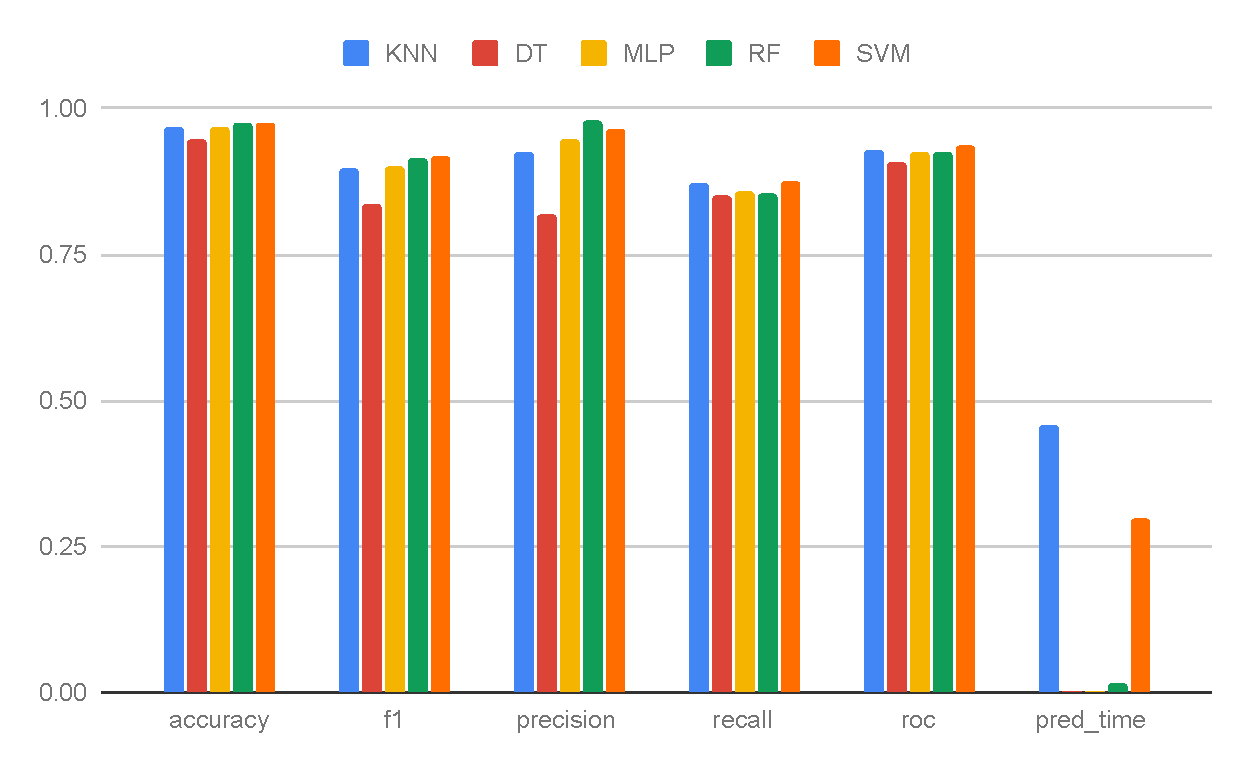
\includegraphics[width=0.9\columnwidth]{media/data/performance/perf_ds_1.pdf}
    \caption{Dataset 1}
    \label{fig:perfromance_results_dataset_1}
  \end{subfigure}%
  % ***************************************** Dataset 2 *****************************************
  \begin{subfigure}{.5\columnwidth}
    \centering
    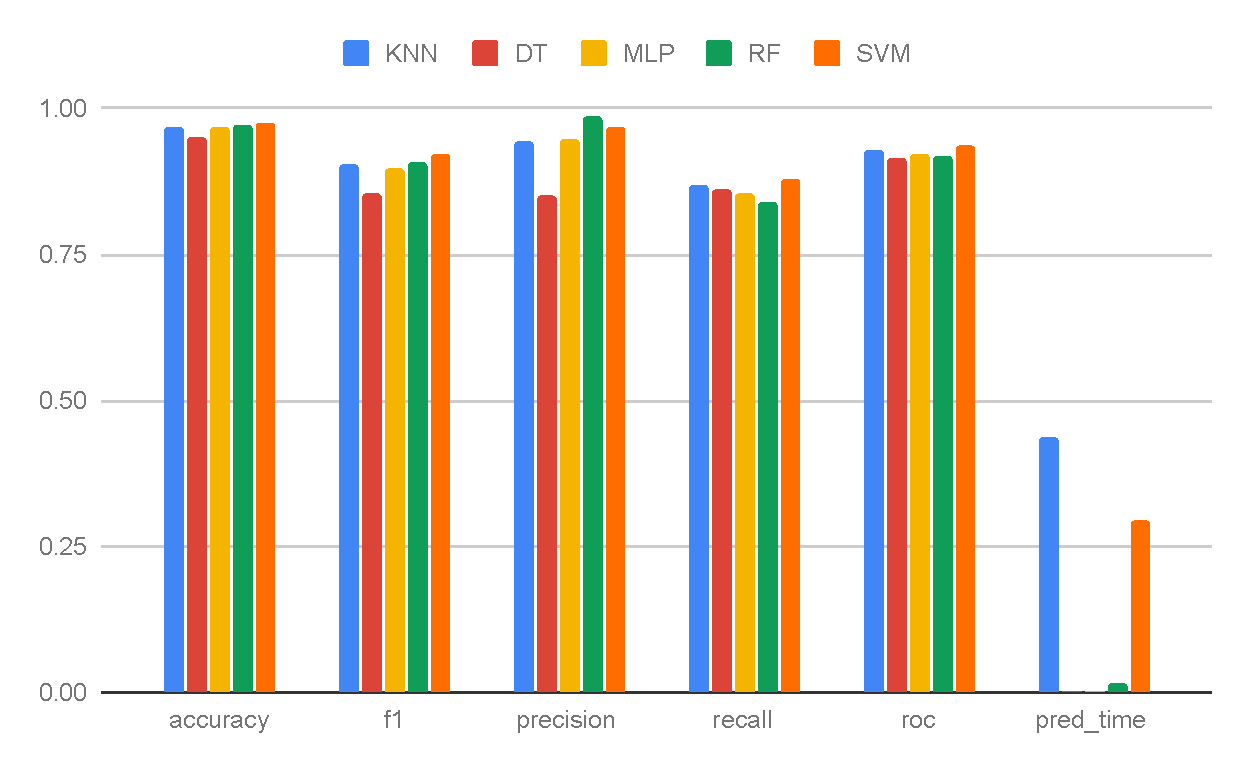
\includegraphics[width=0.9\columnwidth]{media/data/performance/perf_ds_2.pdf}
    \caption{Dataset 2}
    \label{fig:perfromance_results_dataset_2}
  \end{subfigure}\\%
  % ***************************************** Dataset 3 *****************************************
  \begin{subfigure}{.5\columnwidth}
    \centering
    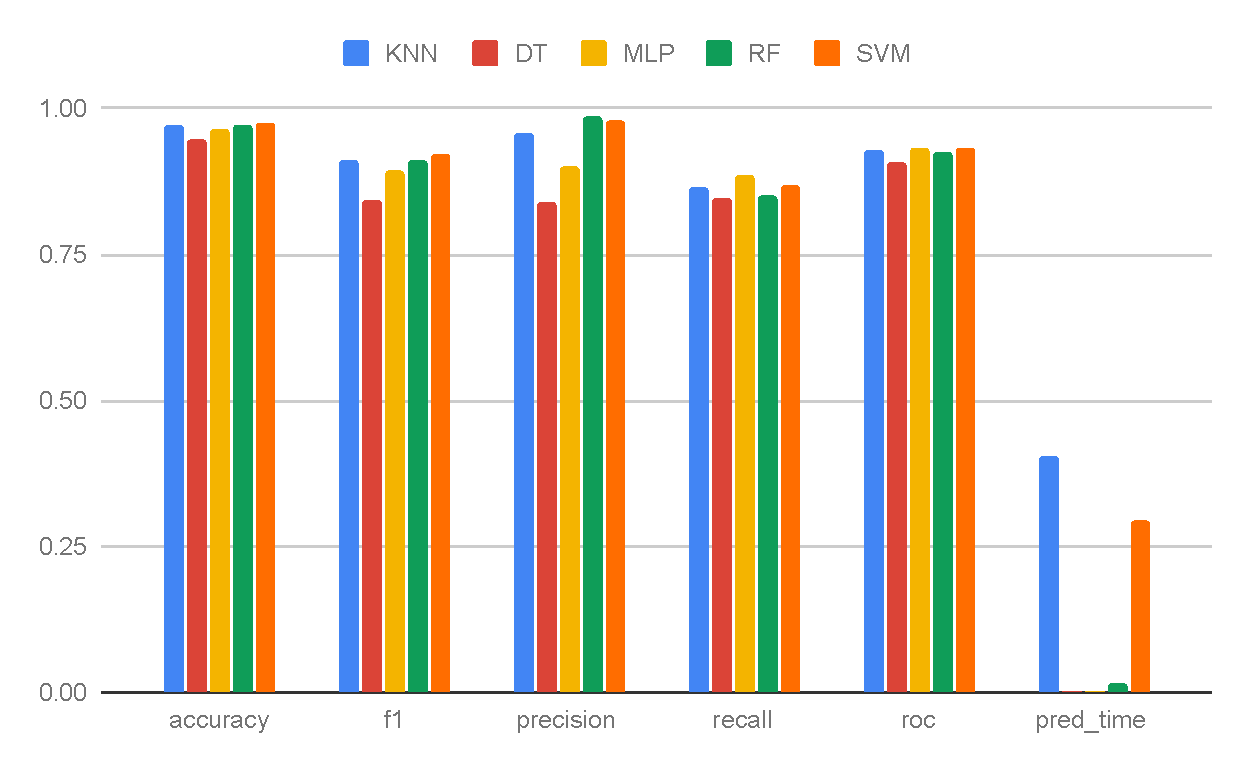
\includegraphics[width=0.9\columnwidth]{media/data/performance/perf_ds_3.pdf}
    \caption{Dataset 3}
    \label{fig:perfromance_results_dataset_3}
  \end{subfigure}%
  % ***************************************** Dataset 4 *****************************************
  \begin{subfigure}{.5\columnwidth}
    \centering
    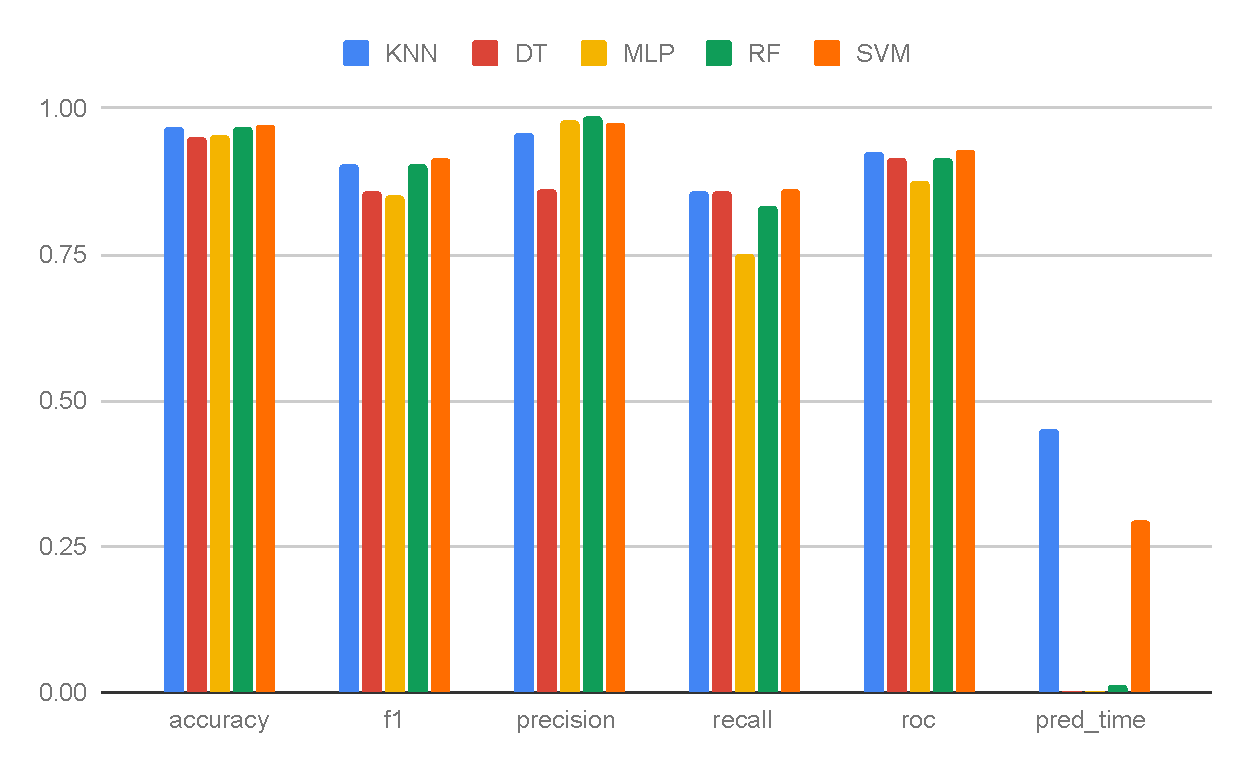
\includegraphics[width=0.9\columnwidth]{media/data/performance/perf_ds_4.pdf}
    \caption{Dataset 4}
    \label{fig:perfromance_results_dataset_4}
  \end{subfigure}
  \caption{Perfromance Results}
  \label{fig:perfromance_results}
\end{figure}

\section{Cross Performance Evaluation} \label{sec:cross_performance_evaluation}

Models tested against other datasets show a slight difference in performance. This difference suggests that the models are capable of performing general predictions. These general tasks can be performed with a small efficiency cost. \Cref{fig:perfromance_delta} shows the performance of models tested on all training datasets.

% *********** Performance delta/performance drop during cross-performance analysis ************
\begin{figure}[H]
  % ******************************************** KNN ********************************************
  \begin{subfigure}{.5\columnwidth}
    \centering
    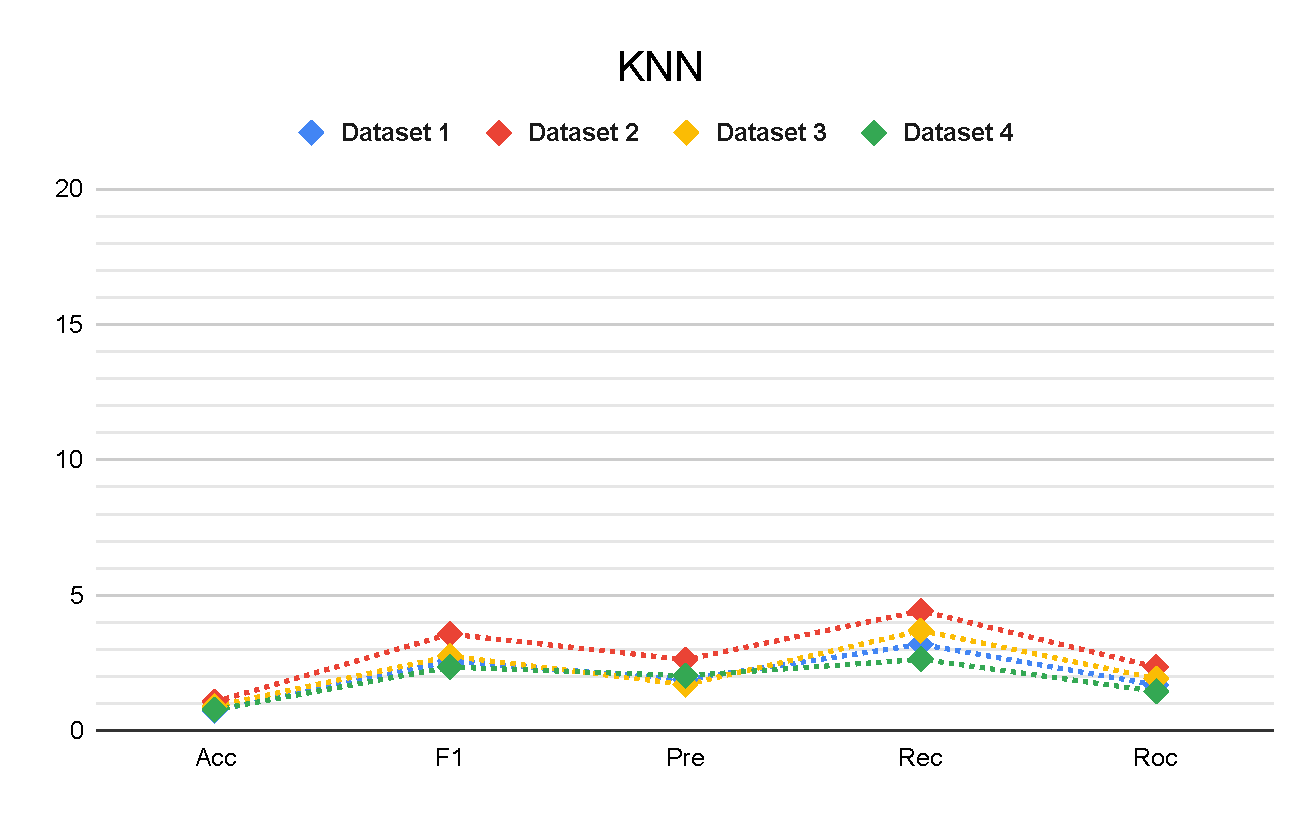
\includegraphics[width=0.9\columnwidth]{media/data/performance_delta/delta_KNN.pdf}
    \caption{}
    \label{fig:perfromance_delta_knn}
  \end{subfigure}%
  % ******************************************** DT *********************************************
  \begin{subfigure}{.5\columnwidth}
    \centering
    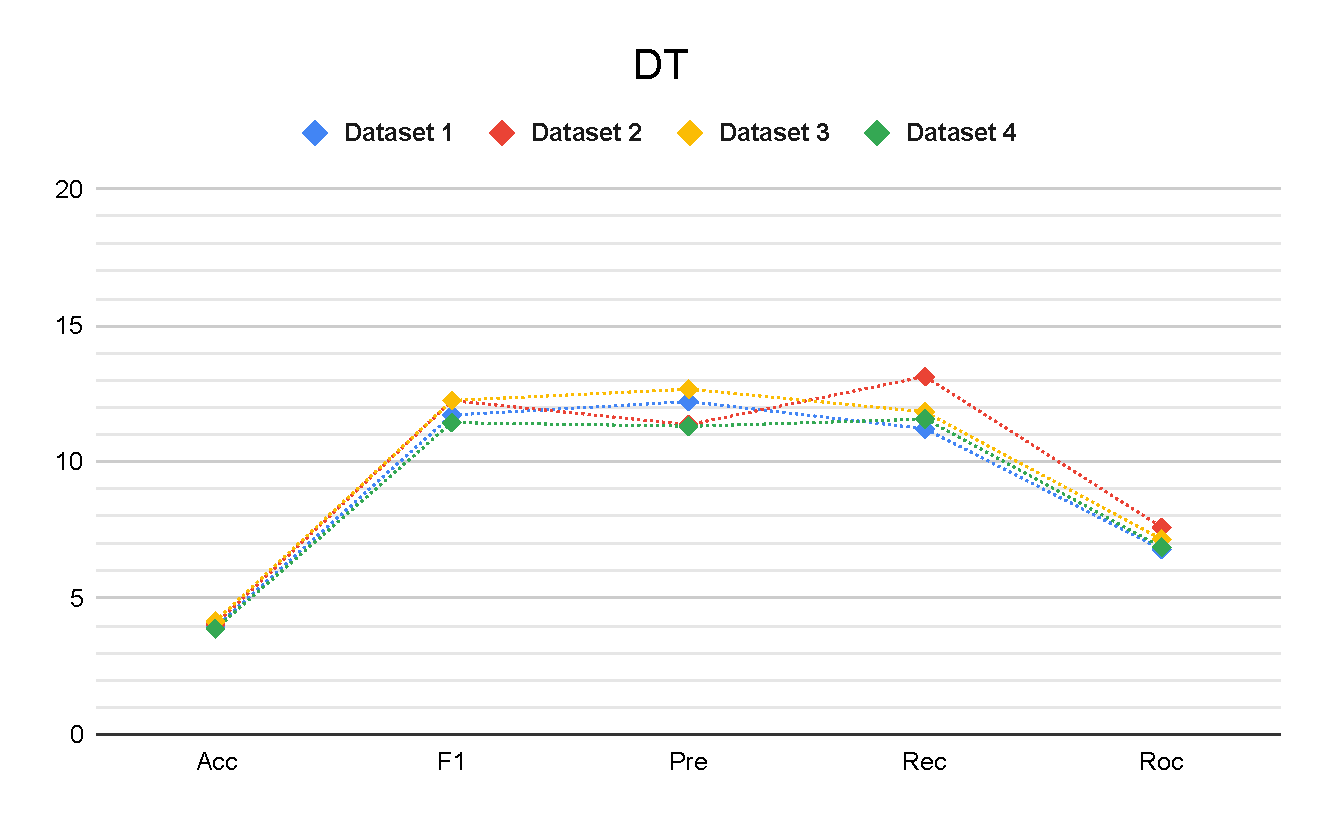
\includegraphics[width=0.9\columnwidth]{media/data/performance_delta/delta_DT.pdf}
    \caption{}
    \label{fig:perfromance_delta_dt}
  \end{subfigure}\\%
  % ******************************************** RF *********************************************
  \begin{subfigure}{.5\columnwidth}
    \centering
    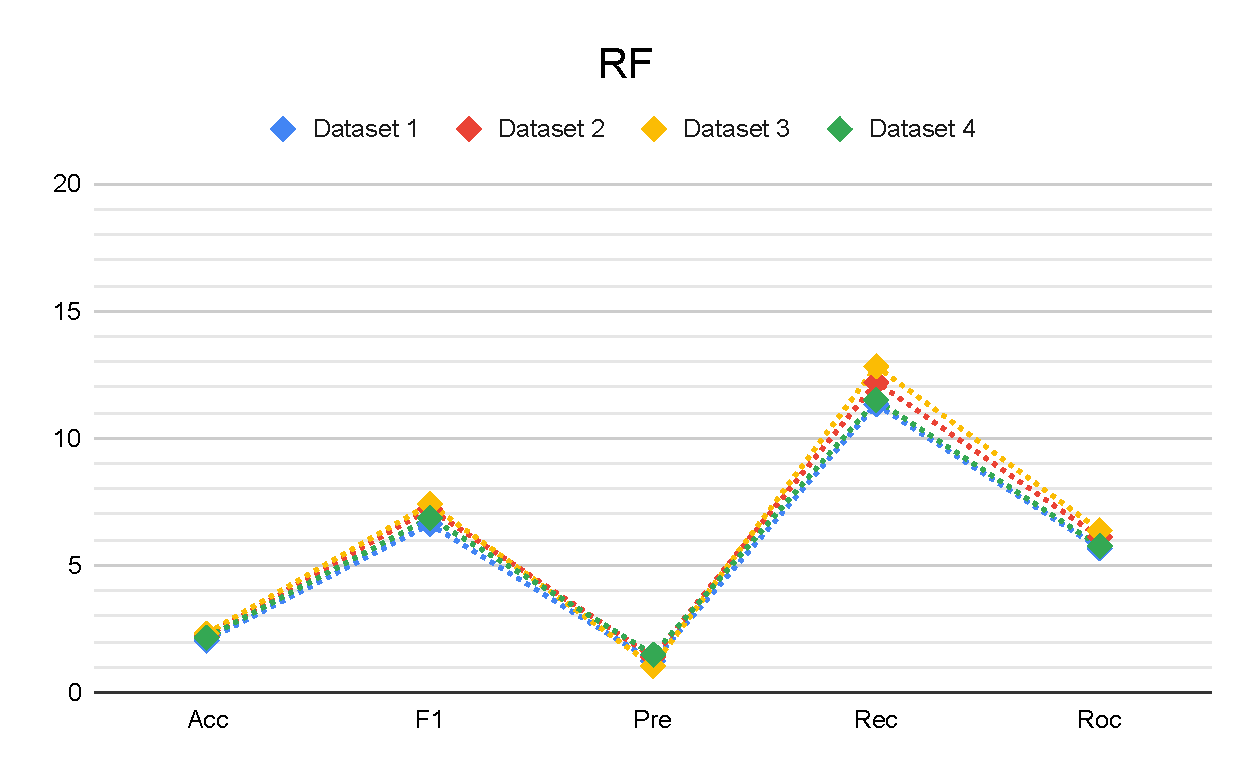
\includegraphics[width=0.9\columnwidth]{media/data/performance_delta/delta_RF.pdf}
    \caption{}
    \label{fig:perfromance_delta_rf}
  \end{subfigure}%
  % ******************************************** MLP ********************************************
  \begin{subfigure}{.5\columnwidth}
    \centering
    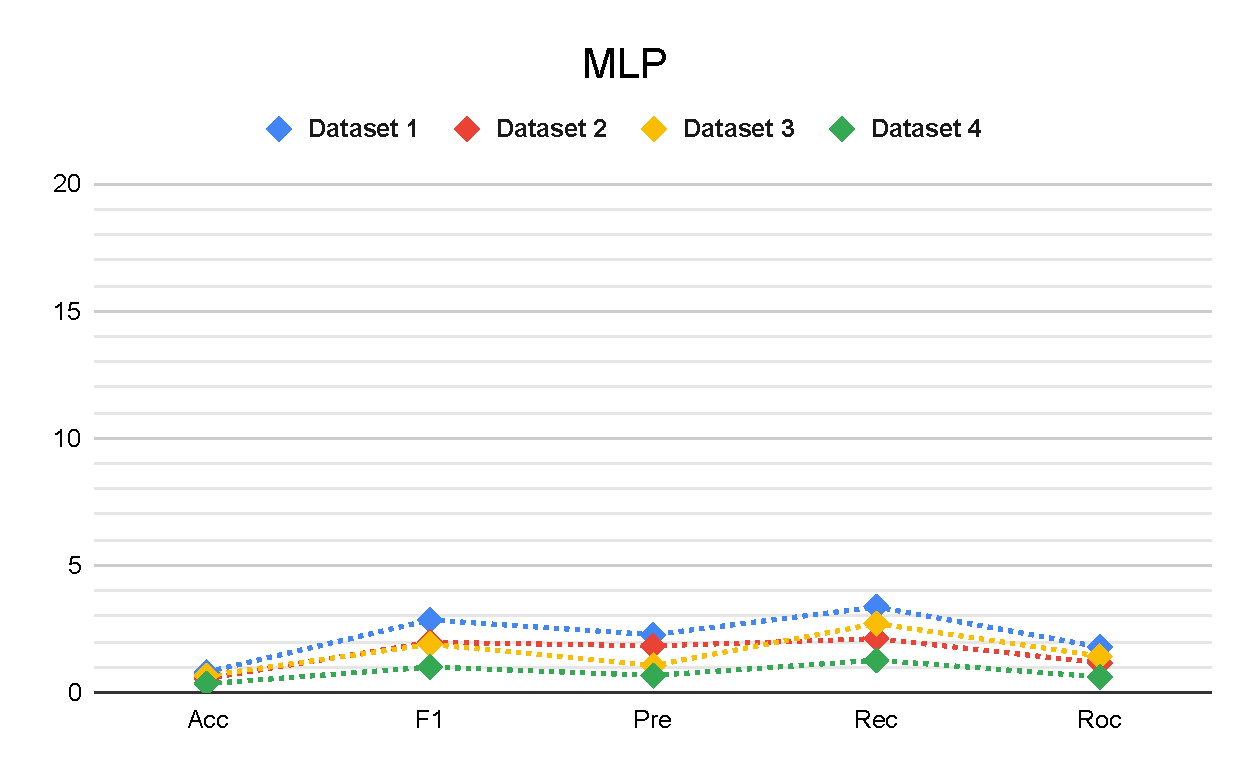
\includegraphics[width=0.9\columnwidth]{media/data/performance_delta/delta_MLP.pdf}
    \caption{}
    \label{fig:perfromance_delta_mlp}
  \end{subfigure}\\%
  % ******************************************** SVM ********************************************
  \begin{subfigure}{.5\columnwidth}
    \centering
    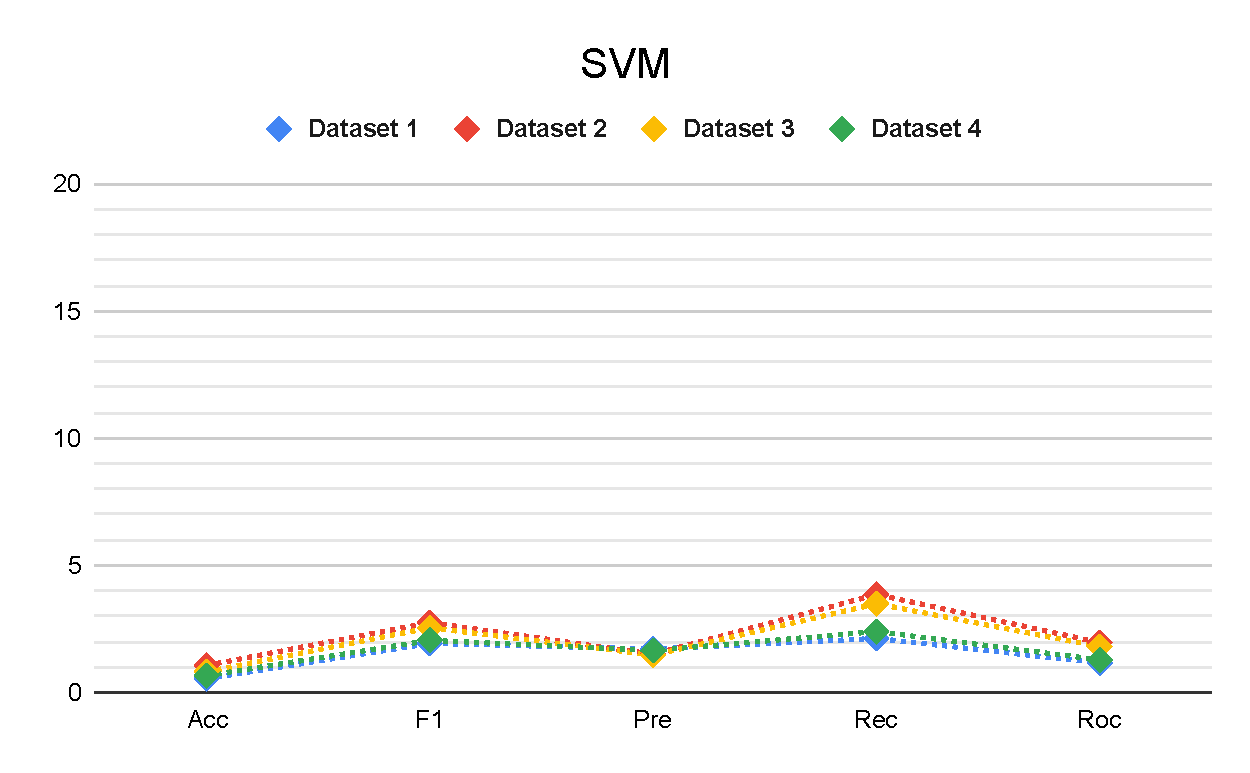
\includegraphics[width=0.9\columnwidth]{media/data/performance_delta/delta_SVM.pdf}
    \caption{}
    \label{fig:perfromance_delta_svm}
  \end{subfigure}
  \caption{Average Perfromance drop}
  \label{fig:perfromance_delta}
\end{figure}

The \cref{fig:perfromance_delta} shows the average performance difference of models concerning training datasets. From \cref{fig:perfromance_delta_dt} and \cref{fig:perfromance_delta_rf}, we can see that the difference in performance metrics of the Decision Tree and Random Forest algorithm is almost similar to all training sets. It indicates that these models can be used as solutions to similar problems. \Cref{fig:perfromance_delta_mlp} shows the maximum difference in performance metrics when tested against other datasets. It indicates that the model is overfitting and is not suitable to be used for other datasets. While \cref{fig:perfromance_delta_knn} and \cref{fig:perfromance_delta_svm} shows good performance metrics for some datasets. This shows models can be tuned for specific requirements. This will produce more satisfactory results in general predictions. \Cref{tab:dt_model_cross-performance_results,tab:knn_model_cross-performance_results,tab:mlp_model_cross-performance_results,tab:rf_model_cross-performance_results,tab:svm_model_cross-performance_results} shows the cross-performance evaluation of models.

% ********************************* cross performance tables **********************************
% ************************************** DT model table ***************************************
\begin{table}[H]
  \centering
  \caption{DT model cross-performance results}\label{tab:dt_model_cross-performance_results}
  \begin{subtable}[H]{0.45\textwidth}
    \centering
    \begin{tabular}{|l|c|c|c|c|}
      \hline
      \textbf{Dataset}   & \textbf{1} & \textbf{2} & \textbf{3} & \textbf{4} \\
      \hline
      \textbf{Accuracy}  & 0.98       & 0.94       & 0.94       & 0.94       \\
      \textbf{F1}        & 0.96       & 0.85       & 0.85       & 0.84       \\
      \textbf{Precision} & 0.95       & 0.83       & 0.84       & 0.83       \\
      \textbf{Recall}    & 0.96       & 0.86       & 0.85       & 0.85       \\
      \textbf{ROC}       & 0.97       & 0.91       & 0.91       & 0.90       \\
      \hline
    \end{tabular}
    \caption{Dataset 1 - DT Model}\label{subtab:dataset_1_dt_model}
  \end{subtable}
  \quad
  \begin{subtable}[H]{0.45\textwidth}
    \centering
    \begin{tabular}{|l|c|c|c|c|}
      \hline
      \textbf{Dataset}   & \textbf{1} & \textbf{2} & \textbf{3} & \textbf{4} \\
      \hline
      \textbf{Accuracy}  & 0.94       & 0.98       & 0.94       & 0.94       \\
      \textbf{F1}        & 0.84       & 0.96       & 0.84       & 0.85       \\
      \textbf{Precision} & 0.85       & 0.96       & 0.85       & 0.85       \\
      \textbf{Recall}    & 0.82       & 0.96       & 0.84       & 0.84       \\
      \textbf{ROC}       & 0.89       & 0.97       & 0.90       & 0.90       \\
      \hline
    \end{tabular}
    \caption{Dataset 2 - DT Model}\label{subtab:dataset_2_dt_model}
  \end{subtable}
  \quad
  \begin{subtable}[H]{0.45\textwidth}
    \centering
    \begin{tabular}{|l|c|c|c|c|}
      \hline
      \textbf{Dataset}   & \textbf{1} & \textbf{2} & \textbf{3} & \textbf{4} \\
      \hline
      \textbf{Accuracy}  & 0.94       & 0.94       & 0.98       & 0.94       \\
      \textbf{F1}        & 0.84       & 0.84       & 0.96       & 0.83       \\
      \textbf{Precision} & 0.84       & 0.83       & 0.95       & 0.83       \\
      \textbf{Recall}    & 0.84       & 0.85       & 0.96       & 0.84       \\
      \textbf{ROC}       & 0.90       & 0.90       & 0.97       & 0.90       \\
      \hline
    \end{tabular}
    \caption{Dataset 3 - DT Model}\label{subtab:dataset_3_dt_model}
  \end{subtable}
  \quad
  \begin{subtable}[H]{0.45\textwidth}
    \centering
    \begin{tabular}{|l|c|c|c|c|}
      \hline
      \textbf{Dataset}   & \textbf{1} & \textbf{2} & \textbf{3} & \textbf{4} \\
      \hline
      \textbf{Accuracy}  & 0.94       & 0.94       & 0.95       & 0.98       \\
      \textbf{F1}        & 0.85       & 0.85       & 0.85       & 0.96       \\
      \textbf{Precision} & 0.85       & 0.85       & 0.85       & 0.96       \\
      \textbf{Recall}    & 0.85       & 0.84       & 0.85       & 0.96       \\
      \textbf{ROC}       & 0.91       & 0.90       & 0.91       & 0.97       \\
      \hline
    \end{tabular}
    \caption{Dataset 4 - DT Model}\label{subtab:dataset_4_dt_model}
  \end{subtable}
\end{table}

% ************************************** KNN model table **************************************
\begin{table}[H]
  \centering
  \caption{KNN model cross-performance results}\label{tab:knn_model_cross-performance_results}
  \begin{subtable}[H]{0.45\textwidth}
    \centering
    \begin{tabular}{|l|c|c|c|c|}
      \hline
      \textbf{Dataset}   & \textbf{1} & \textbf{2} & \textbf{3} & \textbf{4} \\
      \hline
      \textbf{Accuracy}  & 0.97       & 0.97       & 0.97       & 0.96       \\
      \textbf{F1}        & 0.93       & 0.91       & 0.90       & 0.90       \\
      \textbf{Precision} & 0.96       & 0.95       & 0.94       & 0.94       \\
      \textbf{Recall}    & 0.90       & 0.87       & 0.87       & 0.87       \\
      \textbf{ROC}       & 0.94       & 0.93       & 0.93       & 0.93       \\
      \hline
    \end{tabular}
    \caption{Dataset 1 - KNN Model}\label{subtab:dataset_1_knn_model}
  \end{subtable}
  \quad
  \begin{subtable}[H]{0.45\textwidth}
    \centering
    \begin{tabular}{|l|c|c|c|c|}
      \hline
      \textbf{Dataset}   & \textbf{1} & \textbf{2} & \textbf{3} & \textbf{4} \\
      \hline
      \textbf{Accuracy}  & 0.96       & 0.97       & 0.96       & 0.96       \\
      \textbf{F1}        & 0.90       & 0.93       & 0.90       & 0.89       \\
      \textbf{Precision} & 0.94       & 0.96       & 0.94       & 0.94       \\
      \textbf{Recall}    & 0.86       & 0.90       & 0.86       & 0.85       \\
      \textbf{ROC}       & 0.92       & 0.94       & 0.92       & 0.92       \\
      \hline
    \end{tabular}
    \caption{Dataset 2 - KNN Model}\label{subtab:dataset_2_knn_model}
  \end{subtable}
  \quad
  \begin{subtable}[H]{0.45\textwidth}
    \centering
    \begin{tabular}{|l|c|c|c|c|}
      \hline
      \textbf{Dataset}   & \textbf{1} & \textbf{2} & \textbf{3} & \textbf{4} \\
      \hline
      \textbf{Accuracy}  & 0.96       & 0.96       & 0.97       & 0.96       \\
      \textbf{F1}        & 0.90       & 0.90       & 0.93       & 0.90       \\
      \textbf{Precision} & 0.95       & 0.95       & 0.96       & 0.94       \\
      \textbf{Recall}    & 0.86       & 0.86       & 0.89       & 0.86       \\
      \textbf{ROC}       & 0.92       & 0.92       & 0.94       & 0.92       \\
      \hline
    \end{tabular}
    \caption{Dataset 3 - KNN Model}\label{subtab:dataset_3_knn_model}
  \end{subtable}
  \quad
  \begin{subtable}[H]{0.45\textwidth}
    \centering
    \begin{tabular}{|l|c|c|c|c|}
      \hline
      \textbf{Dataset}   & \textbf{1} & \textbf{2} & \textbf{3} & \textbf{4} \\
      \hline
      \textbf{Accuracy}  & 0.96       & 0.96       & 0.96       & 0.97       \\
      \textbf{F1}        & 0.90       & 0.90       & 0.90       & 0.92       \\
      \textbf{Precision} & 0.94       & 0.95       & 0.94       & 0.96       \\
      \textbf{Recall}    & 0.86       & 0.86       & 0.87       & 0.89       \\
      \textbf{ROC}       & 0.92       & 0.92       & 0.93       & 0.94       \\
      \hline
    \end{tabular}
    \caption{Dataset 4 - KNN Model}\label{subtab:dataset_4_knn_model}
  \end{subtable}
\end{table}

% ************************************** MLP model table **************************************
\begin{table}[H]
  \centering
  \caption{MLP model cross-performance results}\label{tab:mlp_model_cross-performance_results}
  \begin{subtable}[H]{0.45\textwidth}
    \centering
    \begin{tabular}{|l|c|c|c|c|}
      \hline
      \textbf{Dataset}   & \textbf{1} & \textbf{2} & \textbf{3} & \textbf{4} \\
      \hline
      \textbf{Accuracy}  & 0.97       & 0.96       & 0.96       & 0.96       \\
      \textbf{F1}        & 0.92       & 0.89       & 0.89       & 0.89       \\
      \textbf{Precision} & 0.97       & 0.95       & 0.94       & 0.95       \\
      \textbf{Recall}    & 0.88       & 0.85       & 0.85       & 0.85       \\
      \textbf{ROC}       & 0.93       & 0.92       & 0.92       & 0.92       \\
      \hline
    \end{tabular}
    \caption{Dataset 1 - MLP Model}\label{subtab:dataset_1_mlp_model}
  \end{subtable}
  \quad
  \begin{subtable}[H]{0.45\textwidth}
    \centering
    \begin{tabular}{|l|c|c|c|c|}
      \hline
      \textbf{Dataset}   & \textbf{1} & \textbf{2} & \textbf{3} & \textbf{4} \\
      \hline
      \textbf{Accuracy}  & 0.96       & 0.97       & 0.96       & 0.96       \\
      \textbf{F1}        & 0.90       & 0.91       & 0.90       & 0.90       \\
      \textbf{Precision} & 0.95       & 0.97       & 0.94       & 0.95       \\
      \textbf{Recall}    & 0.85       & 0.87       & 0.85       & 0.85       \\
      \textbf{ROC}       & 0.92       & 0.93       & 0.92       & 0.92       \\
      \hline
    \end{tabular}
    \caption{Dataset 2 - MLP Model}\label{subtab:dataset_2_mlp_model}
  \end{subtable}
  \quad
  \begin{subtable}[H]{0.45\textwidth}
    \centering
    \begin{tabular}{|l|c|c|c|c|}
      \hline
      \textbf{Dataset}   & \textbf{1} & \textbf{2} & \textbf{3} & \textbf{4} \\
      \hline
      \textbf{Accuracy}  & 0.96       & 0.96       & 0.96       & 0.96       \\
      \textbf{F1}        & 0.89       & 0.89       & 0.90       & 0.88       \\
      \textbf{Precision} & 0.89       & 0.89       & 0.90       & 0.89       \\
      \textbf{Recall}    & 0.88       & 0.88       & 0.91       & 0.88       \\
      \textbf{ROC}       & 0.93       & 0.93       & 0.94       & 0.93       \\
      \hline
    \end{tabular}
    \caption{Dataset 3 - MLP Model}\label{subtab:dataset_3_mlp_model}
  \end{subtable}
  \quad
  \begin{subtable}[H]{0.45\textwidth}
    \centering
    \begin{tabular}{|l|c|c|c|c|}
      \hline
      \textbf{Dataset}   & \textbf{1} & \textbf{2} & \textbf{3} & \textbf{4} \\
      \hline
      \textbf{Accuracy}  & 0.95       & 0.95       & 0.95       & 0.95       \\
      \textbf{F1}        & 0.85       & 0.85       & 0.85       & 0.86       \\
      \textbf{Precision} & 0.97       & 0.97       & 0.97       & 0.98       \\
      \textbf{Recall}    & 0.75       & 0.75       & 0.75       & 0.76       \\
      \textbf{ROC}       & 0.87       & 0.87       & 0.87       & 0.88       \\
      \hline
    \end{tabular}
    \caption{Dataset 4 - MLP Model}\label{subtab:dataset_4_mlp_model}
  \end{subtable}
\end{table}

% ************************************** RF model table **************************************
\begin{table}[H]
  \centering
  \caption{RF model cross-performance results}\label{tab:rf_model_cross-performance_results}
  \begin{subtable}[H]{0.45\textwidth}
    \centering
    \begin{tabular}{|l|c|c|c|c|}
      \hline
      \textbf{Dataset}   & \textbf{1} & \textbf{2} & \textbf{3} & \textbf{4} \\
      \hline
      \textbf{Accuracy}  & 0.99       & 0.97       & 0.97       & 0.97       \\
      \textbf{F1}        & 0.98       & 0.91       & 0.91       & 0.91       \\
      \textbf{Precision} & 0.99       & 0.98       & 0.97       & 0.98       \\
      \textbf{Recall}    & 0.96       & 0.85       & 0.85       & 0.85       \\
      \textbf{ROC}       & 0.98       & 0.92       & 0.92       & 0.92       \\
      \hline
    \end{tabular}
    \caption{Dataset 1 - RF Model}\label{subtab:dataset_1_rf_model}
  \end{subtable}
  \quad
  \begin{subtable}[H]{0.45\textwidth}
    \centering
    \begin{tabular}{|l|c|c|c|c|}
      \hline
      \textbf{Dataset}   & \textbf{1} & \textbf{2} & \textbf{3} & \textbf{4} \\
      \hline
      \textbf{Accuracy}  & 0.96       & 0.99       & 0.97       & 0.97       \\
      \textbf{F1}        & 0.90       & 0.97       & 0.91       & 0.90       \\
      \textbf{Precision} & 0.98       & 0.99       & 0.97       & 0.98       \\
      \textbf{Recall}    & 0.83       & 0.96       & 0.85       & 0.84       \\
      \textbf{ROC}       & 0.91       & 0.98       & 0.92       & 0.91       \\
      \hline
    \end{tabular}
    \caption{Dataset 2 - RF Model}\label{subtab:dataset_2_rf_model}
  \end{subtable}
  \quad
  \begin{subtable}[H]{0.45\textwidth}
    \centering
    \begin{tabular}{|l|c|c|c|c|}
      \hline
      \textbf{Dataset}   & \textbf{1} & \textbf{2} & \textbf{3} & \textbf{4} \\
      \hline
      \textbf{Accuracy}  & 0.96       & 0.97       & 0.99       & 0.97       \\
      \textbf{F1}        & 0.90       & 0.90       & 0.97       & 0.90       \\
      \textbf{Precision} & 0.98       & 0.98       & 0.99       & 0.98       \\
      \textbf{Recall}    & 0.83       & 0.84       & 0.96       & 0.83       \\
      \textbf{ROC}       & 0.91       & 0.91       & 0.98       & 0.91       \\
      \hline
    \end{tabular}
    \caption{Dataset 3 - RF Model}\label{subtab:dataset_3_rf_model}
  \end{subtable}
  \quad
  \begin{subtable}[H]{0.45\textwidth}
    \centering
    \begin{tabular}{|l|c|c|c|c|}
      \hline
      \textbf{Dataset}   & \textbf{1} & \textbf{2} & \textbf{3} & \textbf{4} \\
      \hline
      \textbf{Accuracy}  & 0.96       & 0.97       & 0.97       & 0.99       \\
      \textbf{F1}        & 0.90       & 0.91       & 0.90       & 0.97       \\
      \textbf{Precision} & 0.98       & 0.98       & 0.97       & 0.99       \\
      \textbf{Recall}    & 0.84       & 0.84       & 0.85       & 0.95       \\
      \textbf{ROC}       & 0.91       & 0.92       & 0.92       & 0.97       \\
      \hline
    \end{tabular}
    \caption{Dataset 4 - RF Model}\label{subtab:dataset_4_rf_model}
  \end{subtable}
\end{table}

% ************************************** SVM model table **************************************
\begin{table}[H]
  \centering
  \caption{SVM model cross-performance results}\label{tab:svm_model_cross-performance_results}
  \begin{subtable}[H]{0.45\textwidth}
    \centering
    \begin{tabular}{|l|c|c|c|c|}
      \hline
      \textbf{Dataset}   & \textbf{1} & \textbf{2} & \textbf{3} & \textbf{4} \\
      \hline
      \textbf{Accuracy}  & 0.97       & 0.97       & 0.97       & 0.97       \\
      \textbf{F1}        & 0.93       & 0.92       & 0.91       & 0.91       \\
      \textbf{Precision} & 0.98       & 0.97       & 0.96       & 0.96       \\
      \textbf{Recall}    & 0.89       & 0.87       & 0.87       & 0.87       \\
      \textbf{ROC}       & 0.94       & 0.93       & 0.93       & 0.93       \\
      \hline
    \end{tabular}
    \caption{Dataset 1 - SVM Model}\label{subtab:dataset_1_svm_model}
  \end{subtable}
  \quad
  \begin{subtable}[H]{0.45\textwidth}
    \centering
    \begin{tabular}{|l|c|c|c|c|}
      \hline
      \textbf{Dataset}   & \textbf{1} & \textbf{2} & \textbf{3} & \textbf{4} \\
      \hline
      \textbf{Accuracy}  & 0.97       & 0.98       & 0.97       & 0.97       \\
      \textbf{F1}        & 0.91       & 0.94       & 0.91       & 0.91       \\
      \textbf{Precision} & 0.97       & 0.98       & 0.96       & 0.96       \\
      \textbf{Recall}    & 0.86       & 0.89       & 0.86       & 0.86       \\
      \textbf{ROC}       & 0.92       & 0.94       & 0.93       & 0.92       \\
      \hline
    \end{tabular}
    \caption{Dataset 2 - SVM Model}\label{subtab:dataset_2_svm_model}
  \end{subtable}
  \quad
  \begin{subtable}[H]{0.45\textwidth}
    \centering
    \begin{tabular}{|l|c|c|c|c|}
      \hline
      \textbf{Dataset}   & \textbf{1} & \textbf{2} & \textbf{3} & \textbf{4} \\
      \hline
      \textbf{Accuracy}  & 0.97       & 0.97       & 0.98       & 0.97       \\
      \textbf{F1}        & 0.91       & 0.92       & 0.94       & 0.91       \\
      \textbf{Precision} & 0.97       & 0.97       & 0.98       & 0.97       \\
      \textbf{Recall}    & 0.85       & 0.87       & 0.89       & 0.87       \\
      \textbf{ROC}       & 0.92       & 0.93       & 0.94       & 0.93       \\
      \hline
    \end{tabular}
    \caption{Dataset 3 - SVM Model}\label{subtab:dataset_3_svm_model}
  \end{subtable}
  \quad
  \begin{subtable}[H]{0.45\textwidth}
    \centering
    \begin{tabular}{|l|c|c|c|c|}
      \hline
      \textbf{Dataset}   & \textbf{1} & \textbf{2} & \textbf{3} & \textbf{4} \\
      \hline
      \textbf{Accuracy}  & 0.97       & 0.97       & 0.97       & 0.97       \\
      \textbf{F1}        & 0.91       & 0.91       & 0.91       & 0.93       \\
      \textbf{Precision} & 0.97       & 0.96       & 0.96       & 0.98       \\
      \textbf{Recall}    & 0.85       & 0.86       & 0.86       & 0.88       \\
      \textbf{ROC}       & 0.92       & 0.93       & 0.93       & 0.94       \\
      \hline
    \end{tabular}
    \caption{Dataset 4 - SVM Model}\label{subtab:dataset_4_svm_model}
  \end{subtable}
\end{table}

% *********************************************************************************************
% ******************************* Discarded code for future use *******************************
% *********************************************************************************************
%
% ************************************** model peformance *************************************
%
% \begin{table}[H]
%     \centering
%     \caption{Performance of models trained on following datasets}\label{tab:performance_of_models_trained_on_following_datasets}
%         \begin{subtable}[H]{0.9\textwidth}
%             \centering
%             \begin{tabular}{|p{5em}|C{3em}|C{3em}|C{3em}|C{3em}|C{3em}|}
%                 \hline
%                 \textbf{Metric} & \textbf{KNN} & \textbf{DT} & \textbf{MLP} & \textbf{RF} & \textbf{SVM} \\
%                 \hline
%                 \textbf{Accuracy} & 96.72 & 94.46 & 96.89 & 97.33 & \textbf{97.40} \\
%                 \textbf{F1} & 89.71 & 83.43 & 90.05 & 91.30 & \textbf{91.69} \\
%                 \textbf{Precision} & 92.53 & 81.86 & 94.71 & 97.95 & \textbf{96.43} \\
%                 \textbf{Recall} & 87.06 & 85.06 & 85.84 & 85.50 & \textbf{87.40} \\
%                 \textbf{ROC} & 92.84 & 90.68 & 92.45 & 92.57 & \textbf{93.38} \\
%                 \textbf{Time(s)} & 0.457 & 0.001 & 0.002 & 0.015 & \textbf{0.297} \\
%                 \hline
%             \end{tabular}
%             \caption{Dataset 1}\label{tab:performance_of_models_trained_on_dataset_1}
%         \end{subtable}
%     \begin{subtable}[H]{0.9\textwidth}
%         \centering
%         \begin{tabular}{|p{5em}|C{3em}|C{3em}|C{3em}|C{3em}|C{3em}|}
%             \hline
%             \textbf{Metric} & \textbf{KNN} & \textbf{DT} & \textbf{MLP} & \textbf{RF} & \textbf{SVM} \\
%             \hline
%             \textbf{Accuracy} & 96.83 & 95.04 & 96.69 & 97.09 & \textbf{97.46} \\
%             \textbf{F1} & 90.28 & 85.50 & 89.73 & 90.75 & \textbf{92.15} \\
%             \textbf{Precision} & 94.25 & 84.90 & 94.73 & 98.60 & \textbf{96.79} \\
%             \textbf{Recall} & 86.63 & 86.09 & 85.23 & 84.05 & \textbf{87.93} \\
%             \textbf{ROC} & 92.77 & 91.48 & 92.13 & 91.90 & \textbf{93.66} \\
%             \textbf{Time(s)} & 0.435 & 0.001 & 0.003 & 0.014 & \textbf{0.295} \\
%             \hline
%         \end{tabular}
%         \caption{Dataset 2}\label{subtab:models_trained_on_dataset_2}
%     \end{subtable}
%     \quad
%     \begin{subtable}[H]{0.9\textwidth}
%         \centering
%         \begin{tabular}{|p{5em}|C{3em}|C{3em}|C{3em}|C{3em}|C{3em}|}
%             \hline
%             \textbf{Metric} & \textbf{KNN} & \textbf{DT} & \textbf{MLP} & \textbf{RF} & \textbf{SVM} \\
%             \hline
%             \textbf{Accuracy} & 97.07 & 94.64 & 96.41 & \textbf{97.22} & 97.44 \\
%             \textbf{F1} & 90.93 & 84.30 & 89.34 & \textbf{91.21} & 92.00 \\
%             \textbf{Precision} & 95.82 & 83.81 & 90.13 & \textbf{98.37} & 97.81 \\
%             \textbf{Recall} & 86.53 & 84.80 & 88.57 & \textbf{85.02} & 86.85 \\
%             \textbf{ROC} & 92.87 & 90.73 & 93.29 & \textbf{92.36} & 93.22 \\
%             \textbf{Time(s)} & 0.404 & 0.001 & 0.002 & \textbf{0.017} & 0.293 \\
%             \hline
%         \end{tabular}
%         \caption{Dataset 3}\label{subtab:models_trained_on_dataset_3}
%     \end{subtable}
%     \quad
%     \begin{subtable}[H]{0.9\textwidth}
%         \centering
%         \begin{tabular}{|p{5em}|C{3em}|C{3em}|C{3em}|C{3em}|C{3em}|}
%             \hline
%             \textbf{Metric} & \textbf{KNN} & \textbf{DT} & \textbf{MLP} & \textbf{RF} & \textbf{SVM} \\
%             \hline
%             \textbf{Accuracy} & 96.84 & 94.99 & 95.34 & 96.88 & \textbf{97.15} \\
%             \textbf{F1} & 90.52 & 85.73 & 85.01 & 90.37 & \textbf{91.39} \\
%             \textbf{Precision} & 95.71 & 85.91 & 97.83 & 98.65 & \textbf{97.41} \\
%             \textbf{Recall} & 85.86 & 85.55 & 75.15 & 83.37 & \textbf{86.07} \\
%             \textbf{ROC} & 92.52 & 91.28 & 87.40 & 91.56 & \textbf{92.79} \\
%             \textbf{Time(s)} & 0.452 & 0.001 & 0.002 & 0.014 & \textbf{0.294} \\
%             \hline
%         \end{tabular}
%         \caption{Dataset 4}\label{subtab:models_trained_on_dataset_4}
%     \end{subtable}
% \end{table}
%
% ******************************************** End ********************************************
\thispagestyle{fancy}
\chapter{Applications} \label{ch:applications}
\section*{\centering Chapter \thechapter}
\section*{\centering Applications}

The application is intended to be used by medical staff in COVID-19 wards. It is primarily
built to detect arrhythmia in COVID-19 patients.

\section{Detection of Arrhythmia} \label{sec:detection_of_arrhythmia}
In the early phase of the COVID-19 pandemic, the mortality rate was extremely high. It was
partly due to undetected comorbidities in patients. Undetected conditions were the primary
cause of severe cases of COVID-19 infection. These conditions were respiratory disorders,
cardiovascular disorders, diabetic disorders, etc. Earlier detection of these conditions will
help in better case management. The project's application is to detect cardiovascular
disorders. For this purpose, the presence of an arrhythmia can be used as a primary sign.

Arrhythmia can be detected from the patient's ECG reports. This process is automated with the
application of a supervised learning system. This system allows medical staff to train and
select the best-suited model for arrhythmia detection, and help them diagnose such patients.
While the primary goal of this project is to be used in COVID-19 cases, it can also be used for
regular patients.

\section{Detection of anomalies in medical field} \label{sec:detection_of_anomalies_in_medica_field}
Machine learning is widely used for various tasks in the medical field. Supervised learning is
used as diagnosing tool in a few cases. For example, epilepsy is diagnosed by studying scans
obtained from the patient's brain. The proposed system can perform an initial screening to
detect any anomalies. If such an anomaly is present, it will allow medical personnel to
diagnose the patient efficiently.

The application of the system is not limited to diagnosis only, as it can be used for research
purposes. These uses are filtering out unwanted data and detecting anomalies. This anomaly
detection can be used in research data for discovery purposes. This will increase the
productivity of research and lead to rapid development.

\section{Model Training and Predictions} \label{sec:model_training_and_predictions}
The system is capable of training models and selecting models. This system only needs a
well-labeled dataset, and it will automatically select the best model for the task. The system
can be used by a person without any technical or data science knowledge. The training process
can be fine-tuned by adjusting performance weightage. The stored model can be used on similar
datasets for prediction purposes.
\thispagestyle{fancy}
\chapter{Conclusion And Future Scope} \label{ch:conclusion_and_future_scope}
\section*{\centering Chapter \thechapter}
\section*{\centering Conclusion And Future Scope}


\section{Conclusion} \label{sec:conclusion}
As the number of COVID-19 are still increasing, the mortality rate is still rising. The
mortality rate is higher in cases with comorbidities. Cardiovascular diseases are few of the
comorbidities that drive this mortality rate. These diseases can be diagnosed earlier with a
machine learning system. In this project we built an automated model training and selection
system. This system can be used for predicting the presence of arrhythmia, which is the most
common symptom in cardiovascular diseases.

The system uses supervised learning algorithms to generate models. This leads to efficient
training and higher accuracy in predictions. The system can be fine tuned with by users, or it
can be directly used without any formal training. The system showed good performance for
similar datasets, so it can be used for general prediction purposes too.

\section{Future Scope} \label{sec:future_scope}
The current system only provides solutions to binary classification problems, but it can be
used for multiclass classification problems. The provision of user created model templates can
be done, with user provided performance modification. The system can be connected directly to
the hospital servers to train models from patient records directly with the help of the RPA
system.


\phantomsection
\addcontentsline{toc}{chapter}{References}
% \bibliographystyle{IEEEtranN}
\bibliographystyle{cas-model2-names}
\renewcommand\bibname{References}
\renewcommand{\chapter}[2]{}
\section*{\centering References}
\bibliography{0Dissertation.bib}

% \phantomsection
% \chapter*{List of Publications}
\thispagestyle{fancy}
\section*{\centering List of Publications}

\begin{table}[h]
  \centering
  \begin{tabular}{lp{417.25218pt}}
    [1] &
    Y. Ketkar and S. Gawade, ``Effectiveness of Robotic Process Automation for data mining using UiPath'', in \emph{2021 International Conference on Artificial Intelligence and Smart Systems(ICAIS)}. IEEE, 2021,pp. 864--867.
  \end{tabular}
\end{table}

\phantomsection
\addcontentsline{toc}{chapter}{List of Publications}
\chapter*{List of Publications}
\thispagestyle{fancy}
\section*{\centering List of Publications}

\begin{table}[h]
  \centering
  \begin{tabular}{lp{417.25218pt}}
    [1] &
    Y. Ketkar and S. Gawade, ``Effectiveness of Robotic Process Automation for data mining using UiPath'', in \emph{2021 International Conference on Artificial Intelligence and Smart Systems(ICAIS)}. IEEE, 2021,pp. 864--867.
  \end{tabular}
\end{table}

% \pagestyle{empty}
\phantomsection
\addcontentsline{toc}{chapter}{Acknowledgment}
{\centering \bf \LARGE \scshape
Acknowledgement \\
}

\vspace{1em} \noindent
This dissertation report would not have come into reality without the able guidance, support and wishes of all those who stand by me in the  development. I wish to give my special thanks to my guide, \textbf{Dr. Sushopti Gawade}, for his/her timely advice and guidance.

\noindent
I would like to thank our Principal, \textbf{Dr. Sandeep Joshi} for his constant encouragement throughout the course. I humbly thank our M.E Coordinator, \textbf{Dr. Prashant Nitnaware} and our Head of Department, \textbf{Dr. Satishkumar Verma}, for their valuable guidance \& unending support despite a very busy work schedule. The cheerful spirit they radiated all the time fuelled our desire to excel in the work that I had undertaken.

\noindent
I acknowledge all the staff members of the department of Computer Engineering and department of Information Technology for their help and suggestions during various phases of this project work. It's difficult to forget my eminent supporters that are my Friends and Family members who are always there encouraging me in my every deed.

% \vspace{1em} \noindent
% I remain immensely obliged to \textbf{Dr. Sushopti Gawade}, for providing me with the idea of this topic, and for her invaluable support in garnering resource for me either by way of information or computers also her guidance and supervision which made this seminar happen.

% \noindent
% I would like to thank my college Pillai's Institute of Information Technology, New Panvel, our principal \textbf{Dr. Sandeep Joshi}, M.E. Coordinator \textbf{Dr. Prashant Nitnaware} and the H.O.D. of Information Technology Department \textbf{Dr. Satishkumar Varma} for their invaluable support.

% \noindent
% I would like to say that it has indeed been a fulfilling experience for working on this seminar topic.

\vspace{7.5em}
\begin{flushright}
  \begin{tabular}{c}
    \textbf{Yashodhan Prakash Ketkar} \\
  \end{tabular}
\end{flushright}

\end{document}
